%%%%%%%%%%%%%%%%%%%%%%%%%%%%%%%%%%%%%%%%%%%%%%%%%%%%%%%%%%%%%%%%%%%%%%%%%%%%%%%%%%%%%%%%%%%%%%%%%%%%%%%%%%%%%%%%%%%%%%%%%%%%%%%%%%%%%%%%%%%%%%%%%%%%%%%%%%%
% This is just an example/guide for you to refer to when submitting manuscripts to Frontiers, it is not mandatory to use frontiers.cls nor frontiers.tex  %
% This will only generate the Manuscript, the final article will be typeset by Frontier after acceptance.                                                 %
%%%%%%%%%%%%%%%%%%%%%%%%%%%%%%%%%%%%%%%%%%%%%%%%%%%%%%%%%%%%%%%%%%%%%%%%%%%%%%%%%%%%%%%%%%%%%%%%%%%%%%%%%%%%%%%%%%%%%%%%%%%%%%%%%%%%%%%%%%%%%%%%%%%%%%%%%%%

%%% Version 2.0 Generated 2013/09/12 %%%
%%% You will need to have the following packages installed: datetime, fmtcount, etoolbox, fcprefix, which are normally inlcuded in WinEdt. %%%
%%% In http://www.ctan.org/ you can find the packages and how to install them, if necessary. %%%

\makeatletter
\adddialect\l@English\l@english
\makeatother

%\documentclass{frontiersENG} % for Engineering articles
\documentclass[english]{frontiersSCNS} % for Science articles
%\documentclass{frontiersMED} % for Medicine articles

\usepackage{url,lineno}
\linenumbers

\newtheorem{definition}{Definition}

\usepackage{graphicx}
\usepackage[english]{babel}
%It ensures a direct compilation from tex to pdf.
\usepackage{epstopdf}
%\usepackage[sort, numbers, authoryear]{natbib}
\usepackage{listings}
\usepackage{amsmath}
\usepackage{longtable}
\usepackage{url}
\usepackage{flushend}
\usepackage{algorithm}
%\usepackage{algorithmic}
\usepackage{algpseudocode}
%\usepackage{algorithmicx}
\usepackage{caption}% http://ctan.org/pkg/caption
\usepackage{lscape}
\usepackage{subfig}
\usepackage{etoolbox}
\apptocmd{\sloppy}{\hbadness 10000\relax}{}{}


% Leave a blank line between paragraphs in stead of using \\

\copyrightyear{}
\pubyear{}

\def\journal{Neuroinformatics}%%% write here for which journal %%%
\def\DOI{}
\def\articleType{Research Article}
\def\keyFont{\fontsize{8}{11}\helveticabold }
\def\firstAuthorLast{Je\v{z}ek {et~al.}} %use et al only if is more than 1 author
\def\Authors{Petr Je\v{z}ek\,$^{1,2,*}$, Roman Mou\v{c}ek\,$^{1,2}$}
% Affiliations should be keyed to the author's name with superscript numbers and be listed as follows: Laboratory, Institute, Department, Organization, City, State abbreviation (USA, Canada, Australia), and Country (without detailed address information such as city zip codes or street names).
% If one of the authors has a change of address, list the new address below the correspondence details using a superscript symbol and use the same symbol to indicate the author in the author list.
\def\Address{$^{1}$Faculty of Applied Sciences, New Technologies for the Information Society, University of West Bohemia, Plze\v{n}, Czech Republic \\
$^{2}$Faculty of Applied Sciences, Department of Computer Science and Engineering, University of West Bohemia, Plze\v{n}, Czech Republic}
% The Corresponding Author should be marked with an asterisk
% Provide the exact contact address (this time including street name and city zip code) and email of the corresponding author
\def\corrAuthor{Petr Je\v{z}ek}
\def\corrAddress{New Technologies for the Information Society, Department of Computer Science and Engineering, Faculty of Applied Sciences, University of  West Bohemia, Univerzitn\'{i} 8, 306 14  Plze\v{n}, Czech Republic}
\def\corrEmail{jezekp@ntis.zcu.cz}

% \color{FrontiersColor} Is the color used in the Journal name, in the title, and the names of the sections.

\sloppy
\begin{document}
\onecolumn
\firstpage{1}

\title[Semantic Framework for Mapping Object-Oriented Model to Semantic Web Languages]{Semantic Framework for Mapping Object-Oriented Model to Semantic Web Languages}
\author[\firstAuthorLast]{\Authors}
\address{}
\correspondance{}
\extraAuth{}% If there are more than 1 corresponding author, comment this line and uncomment the next one.
%\extraAuth{corresponding Author2 \\ Laboratory X2, Institute X2, Department X2, Organization X2, Street X2, City X2 , State XX2 (only USA, Canada and Australia), Zip Code2, X2 Country X2, email2@uni2.edu}
\topic{}% If your article is part of a Research Topic, please indicate here which.

\maketitle

%%%%%%%%%%%%%%%%%%%%%%%%%%%%%%%%%%%%%%%%%%%%%%%%%%%%%%%%%%%%%%%%%%%%%%%%%%%%%%%%%%%%%%%%%%%%%%%%%%%%%%%%%%%%%%%%%%%%%%%%%%%%%%%%%%%%%%%%%%%%%%%%%%%%%%%%%%%%%%%%%%%%%%%%%%%%%%%%%%%%%%%%%%%%%%%%%%%%%%%%%%%%%%%%%%%%%%%%%%%%%%%%%%%%%%%
%%% The sections below are for reference only.
%%%
%%% For Original Research Articles, Clinical Trial Articles, and Technology Reports the following sections are mandatory:
%%% Abstract, Introduction, Material and Methods, Results, and Discussion.
%%% Please note that the Material and Methods section can be placed in any of the following ways: before Results, before Discussion or after Discussion.
%%%
%%% For Clinical Case Studies the following sections are mandatory: Abstract, Introduction, Background, Discussion, and Concluding Remarks.
%%%
%%% For all other article types there are no mandatory sections.
%%%%%%%%%%%%%%%%%%%%%%%%%%%%%%%%%%%%%%%%%%%%%%%%%%%%%%%%%%%%%%%%%%%%%%%%%%%%%%%%%%%%%%%%%%%%%%%%%%%%%%%%%%%%%%%%%%%%%%%%%%%%%%%%%%%%%%%%%%%%%%%%%%%%%%%%%%%%%%%%%%%%%%%%%%%%%%%%%%%%%%%%%%%%%%%%%%%%%%%%%%%%%%%%%%%%%%%%%%%%%%%%%%%%%%%

\begin{abstract}

%%% Leave the Abstract empty if your article falls under any of the following categories: Editorial Book Review, Commentary, Field Grand Challenge, Opinion or specialty Grand Challenge.
\section{}
  The goal of this article is to contribute to the research efficiency in the electrophysiological domain by improving opportunities for describing semantics of structured electrophysiological data. The research efficiency can be among other measures expressed as an ability of data owners and data users to understand the experimental data in a longer term. It means that the appropriate semantic description of these data is closely related to the success in the long-term management and sharing of data.

  Improvement of data management and sharing requires providing data in standardized data formats and also providing related metadata in standardized semantic structures. The abstract level of such data formats and semantic structures, which is widely discussed in the community, has to be accompanied by selecting suitable semantic expressive means. The article deals with and discusses two main current approaches, use of conventional data structures, repositories, and programming languages one one hand, and use of formal representations of ontologies, known from knowledge representation, such as description logics or semantic web languages on the other hand. Although knowledge engineering offers languages supporting richer semantic expressions and technological advanced approaches, conventional data repositories are still popular among developers, administrators and users because of their simplicity and lower computational complexity. Then the semantics that cannot be expressed in conventional data repositories can be added into the structures of the programming language that accesses and process the described data.

  To cope with this opportunity we introduced a software prototype that enables to add additional and richer semantics into the Java object-oriented code that processes conventional data repositories. A mapping that enables transformation of this code into the Semantic Web language OWL was proposed and implemented as a library - the Semantic Framework. This approach does not burdensome users with additional demands on programming environment since we used reflective Java annotations - metadata added to the Java source code and retrieved at run-time. Moreover, this additional semantics need not to be written by the programmer directly to the code, but it can be collected from non-programmers using a graphic user interface. This approach was validated by integration of the Semantic Framework in the EEG/ERP Portal, together with its registration in the Neuroscience Information Framework.

\tiny
 \keyFont{ \section{Keywords:} electrophysiology, object-oriented code, Semantic Web, ontology, concepts mapping, Semantic Framework} %All article types: you may provide up to 8 keywords; at least 5 are mandatory.
\end{abstract}

\section{Introduction}
\label{intro}

Our research group specializes in research of brain electrical activity and operates a laboratory in which the techniques and methods of electroencephalography (EEG) and event related potentials (ERP) are widely used. In addition to the experimental work, which is mostly focused on recording and analysis of cognitive event related potentials, we are working on the development of the software and hardware infrastructure for research in electrophysiology~\cite{10.3389/fninf.2014.00020}. Our experimental work is typically very time consuming and vast amounts of experimental data are produced at various stages of processing from data recording to their final interpretation, Based on this experience, we know that the means supporting the semantic description of electrophysiological data and also software systems improving the storage, management and sharing of these data (at least within the research group) contribute to a long-term understanding of these data and significantly increase research efficiency. This became more crucial when we decided to share our data, processing steps and workflows within wider community.

The subjects of long-term preservation, quality of semantic description and data sharing itself are of course broadly discussed in the community. A variety of experimental approaches,  techniques and methods, targeted subjects, hardware and software infrastructures etc. used during electrophysiological experiments lead to the accumulation of heterogeneous data in the domain. The semantics of these (and not only these in a general sense) structured data means that they are accompanied by metadata that specify their meaning. Metadata can be usually seen as the links to a~specific dictionary, in which the described data are explained and defined by using e.g. a plain text, sets of values or even formal logic. The richness and accuracy of the semantic content of these dictionaries determines the level of semantic description of data. Then the most pressing difficulties in the domain are not only an absence of standardized and generally used data formats for raw data, but also well-defined metadata and their structures (as described e.g. in~\cite{data-sharing-for-computational-neuroscience}).

In the real world electrophysiological data are stored in numerous, often proprietary, data formats and annotated by metadata differently in both scope and quality sense. Moreover, a number of sophisticated implementations of data repositories including file systems and databases of different types are available. Then the domain data are also annotated respecting limitations of used implementations. If we take into account these conceptual and technological heterogeneities and not give up efforts to increase research efficiency in the field by sharing various computational resources like raw data, metadata, processing methods and workflows among laboratories, then the suitable semantic description of data and the long term management and sharing of data and metadata in the domain are the first important steps to achieve this complex goal.

Then improvement of data sharing requires providing data in standardized (or at least widely used) data formats and providing related metadata in appropriate semantic structures. The abstract level of description of such data formats and metadata structures is currently broadly discussed in the community (e.g. within INCF~\cite{incf} data sharing activities). A well-specified abstract level of these data formats and metadata structures could bring real sharing opportunities in the domain. On the other hand and at the same time one must be careful not to discourage community researchers to provide data and metadata in these formats and structures by introducing them too abstract semantic descriptions. Although this decision is very important for the future of data sharing in the domain, it is not more discussed in this article.

However, any proposed abstract level of the description of the data format and metadata structure in the domain has to be accompanied by selecting expressive means and consequently by selecting technologies that promote desired data sharing. Then another decision between two competing approaches has to be done. The first approach is to use conventional data models and structures and conventional programming languages providing data access. The second approach assumes the usage of formal representations of ontologies, known from knowledge representation field, such as description logic, or Semantic Web languages. It can eventually include reasoning provided by software agents. Discussions of these approaches and their practical applications have been kept for decades. They related mainly to expert systems in the past; currently difficulties and perspectives of the Semantic Web languages and technologies are discussed.

The initial concept of the Semantic Web, as was introduced in~\cite{bernerslee2001semantic}, was based on artificial intelligence techniques; knowledge bases accessed via web interface served for automatic reasoning provided by software agents. However, this approach has been continuously changing since the years 2004--2005 and the Semantic Web started to be more viewed as a large distributed database. This perspective had two following fundamental aspects. The first one is known as the knowledge acquisition bottleneck; acquisition of knowledge is a time consuming process that is made usually by domain experts. As a result, the knowledge bases are rather small comparing to conventional data repositories. This bottleneck is currently even more visible in the context of big data collected from the increasing number and due to technical capabilities of hardware acquisition devices. The second aspect is related to the processing of the conventional data that in most cases does not mean producing entirely new data by reasoning. Data are supposed to be just queried and linked to other data. This view of data is one of the key concepts of linked data~\citep{linked-data}.

The Semantic Web expresses data by a triple-oriented language, Resource Description Framework (RDF)~\citep{wnpx:RDF-PRIMER}. When communities working in knowledge representation and web engineering started to interact more, there was a question if XML as a hierarchically oriented language or RDF as a language supporting graph structures is more suitable for representation of meaning. Finally, XML is used as a mean for the serialization of RDF graphs; RDF/XML documents are created. RDF/XML syntax was the first standardized RDF syntax that it is still widely used. Because expressivity of RDF is limited, W3C\footnote{http://www.w3.org/} defined a more powerful language with more capabilities for expressing meaning, Web Ontology Language (OWL)~\citep{jahrynx:Dean:04:OWO}. The aims of the OWL2 specification are to remove different syntaxes, improve datatype expressivity, provide better organization of imports, and remove difficulties with different versions of OWL syntaxes. While RDF was accepted by a larger community, the OWL language was a large burden for the practical application of the Semantic Web. This language, based on description logic, is usually unintelligible to non-experts. Moreover, not many OWL constructions have been really used in real applications yet. To cope with these difficulties, specific OWL dialects supporting different aspect of the resulting semantic model, are currently available.

The concept of linked data is currently one of four ways to expose RDF data on the web. The other ways include providing SPARQL (SPARQL~\cite{prudhommeaux2008sparql}supported by W3C is the most spread standardized language for queering RDF graphs) endpoints to explore data using SPARQL queries (an example is the RDF platform at~\citep{rdf-platform}), publishing data directly to the web as dump files by using one of the serialization formats for RDF graphs, or using RDFa~\citep{rdfa-core11} for expressing structured data in a markup language (e.g., HTML). The first two approaches are technologically advanced, give users more opportunities to work with data, but they require specific knowledge of developers and administrators and place high demands on hardware equipment. There is also a difficulty with overall availability of SPARQL endpoints (the statistics is provided in~\citep{availability-sparql-endpoints}). As a result, these advanced models serve mainly for initial exploring the contents of the data, while in normal use the data are downloaded (as dump files) and processed locally.

Domain ontologies have been playing a significant role in information systems for a~long time~\citep{747902} and they are well-designed for heterogeneous data description. Originally ontologies were mainly created independently, they did not cope with vast amounts of data and focused on logical reasoning. This approach has bee changing together with the changing view of the Semantic Web. Currently ontologies are created using a bottom-up strategy to take advantage of already existing data. These ontologies are then covered by upper-level ontologies or ontological background models. Since for a newly created dataset we hardly find a comprehensive ontology, there are two basic options (which can be used in parallel), to create an ontology for this new dataset. In the first approach it is supposed to find relevant types of objects and relations in already existing ontologies, compare them, find the most suitable types and reuse them. In the second approach new types are defined, collected and organized in a newly designed ontology. The mixed strategy, when the common types are reused from other ontologies and specific types are newly defined, is for example used during the development of the Ontology for Experimental Neurophysiology (OEN)~\cite{10.3389/conf.fninf.2014.18.00044}. NEMO~\citep{DouFRFMT07} is an ontology describing EEG, averaged EEG (ERPs), and ERP data analysis results; it lacks possibilities to describe experimental protocols and restrictions. It is very complex to be immediately deployed in the electrophysiology domain.

Looking at the semantic expressivity of ontologies from the point of view of the automated processing, the higher the level of formalization is, the easier it is to use the ontology for sharing and reasoning, since it is more machine-processable. On the other hand, it is difficult to develop such an ontology. Moreover, use of formalisms with high expressivity leads to difficulties with decidability and computational complexity when reasoning. Then these formalisms have to be limited in their expressivity to ensure that the resulting ontologies are usable in practice for automated reasoning. Looking at the present state, then despite the increasing popularity of storing data in repositories by using languages providing higher sematic expressivity, most of the data are still stored in conventional repositories such as files and relational databases (a~list of DBMS ranked by their current popularity is available in ~\citep{db-engines}). Taken into account the big conventional data collected from a number of hardware sensors, familiarity of large groups of developers, administrators and users with conventional data repositories, and simplicity of publishing RDF data (transformed from conventional data) as dump files, we can hardly anticipate a substantial change in the use of current types of repositories.

Shared conventional data have often read-only access to third party subjects. It means that only data owners are entitled to add semantics to them. Moreover, conventional relational data repositories due to their limitations in semantic expressivity naturally exclude to add more complex semantic information. However, semantics can be still added later. This can be done by transforming a conventional repository to a semantic repository (e.g. to RDF triple stores) or by semantic enrichment of the conventional programming language that processes data stored in conventional repositories. The first approach is proposed and implemented e.g. by the D2RQ~\citep{efeliksik:bizer2004d2rq} framework that uses a~declarative language to describe a~mapping between a~relational database schema and RDF. However, this solution requires using the SPARQL language for later data access. To avoid using the Semantic Web languages to the last moment and still to cope with opportunities to add richer semantic information it
is necessary to semantically enrich a conventional programming language.

\subsection{Data Models and Programming Tools}
\label{Conventions}

When analyzing several conventional semantic data models~\citep{0720407583, 0126445516}, essentially two following data modeling formalisms are widely used: \emph{the entity-relation (ERA)} model and \emph{object-oriented (OO)} model. Newer formalisms, e.g. \emph{Enhanced-entity�-relationship (EER)} model, only combine these two approaches. The most used language for modelling an application structure, behavior, architecture, business processes and data structures is the Unified Modeling Language (UML). A UML model consists of three major categories (classifiers, events, behaviors) of model elements, each of which may be used to make statements about different kinds of individual things within the system being modeled~\citep{uml25}.

The models defining object types and relations in knowledge engineering are connected with the development of ontologies. Within the Semantic Web languages, RDF is a standard model for data interchange, RDFS is a~language for representing simple RDF vocabularies on the Web, and OWL as a computational logic-based language represents rich and complex knowledge about things, groups of things, and relations between things~\citep{owl-w3c}.

In addition to selecting a data model, we need to select the type of programming language that we use to access the data. As we already mentioned, the Semantic Web languages are not popular for developing application programs~\citep{Semantic_Web_Primer}. The popularity of script-based languages in neuroinformatics continuously rises~\citep{10.3389/neuro.11.014.2009}, but these languages were also not considered to be suitable for the development of large systems~\citep{Scott:2004:PGB:1040231.1040267}. As a result, we selected an object-oriented language, specifically Java, because we can profit from a combination of both object-oriented and semantic concepts by designing a robust object-oriented system storing data in a relational database. A superstructure that provides semantic description of relationships among data is then implemented using the Semantic Web languages.

Semantic Web languages associate three types of features used in the object-oriented world. They describe reality on the conceptual level independent of technological restrictions, i. e. they are similar to UML representations in object oriented programming (OOP). They also constitute a database schema for the base of facts (RDF). Eventually they are processed by software tools in the implemented application, i. e. they are part of the implementation.

Several similarities can be found between UML and OWL. They both have classes, instances or inheritance, enable defining cardinality restrictions, etc. However, in a more detailed view there are many differences between them. The most substantial difference is the meaning of properties and individuals. In UML instances and properties are removed from classes; in OWL, properties are double types; object and datatype properties. The first one links an individual to an individual and the second one links individuals to data values. Next, UML properties always belong to a class, while OWL properties are stand-alone entities. Finally, an understanding of a class extent is also different. While UML classes work inside a program where they are defined, OWL classes provide features to share classes among domains. OWL classes may be defined as a set of individuals which satisfy a restriction expression. Restrictions are two types: either a boolean combination of other classes (\emph{Intersection, Union, Complement}) or a property value restriction on properties (\emph{allValuesFrom, someValuesFrom}).

OWL can discipline names using \emph{AllDifferent}, \emph{SameAs} or \emph{DifferentFrom} constructs. \emph{The Ontology Definition Metamodel} \citep{OMG2009} compares concepts of OWL with the features of UML more in depth. Described differences are summarized in Table~\ref{tab:OWL-and-UML-Features-Comparison} and practically demonstrated in Figure~\ref{fig:umlowlexample}.

\begin{landscape}
% For tables use
\begin{table}
% table caption is above the table
\caption{OWL and UML Features Comparison}
\label{tab:OWL-and-UML-Features-Comparison}       % Give a unique label
% For LaTeX tables use

\begin{tabular}{p{5cm}p{4cm}p{5cm}p{5cm}}
\hline\noalign{\smallskip}
\textbf{UML} & \textbf{OWL} & \textbf{Java} & \textbf{Comment}
\\
\hline\noalign{\smallskip}
Class, atomic type, property ownedAttribute & owl:Class & \emph{class} &
\\
\hline\noalign{\smallskip}
instance & individual & class instance & OWL owl:individual class independent
\\
\hline\noalign{\smallskip}
owned attribute, association & owl:DataTypeProperty, owl:ObjectProperty & class attributes: primitive data types/objects & OWL has only global attributes
\\
\hline\noalign{\smallskip}

subclass, generalization & owl:subclass, owl:subproperty & \emph{extends}, inherited classes and properties & Java does not support multiple inheritance
\\
\hline\noalign{\smallskip}

enumeration & owl:oneOf & \emph{enum} &
\\
\hline\noalign{\smallskip}

disjoint & owl:disjointWith, owl:unionOf & One object always an instance of exactly one class, but we should pay attention to class inheritance &
\\
\hline\noalign{\smallskip}

multiplicity & owl:MinCardinality, owl:MaxCardinality & \multicolumn{1}{c}{---} &
\\
\hline\noalign{\smallskip}

package & ontology & \emph{package} &
\\
\hline\noalign{\smallskip}
dependency & RDF:property & methods parameters or return value &
\\
\hline\noalign{\smallskip}
\multicolumn{1}{c}{---} & owl:intersectionOf, owl:unionOf, owl:complementOf, owl:DifferentFrom, owl:AllDifferentFrom, owl:allValuesFrom, owl:someValuesFrom, owl:SameAs & \multicolumn{1}{c}{---} &
\\
\hline\noalign{\smallskip}
\end{tabular}

\end{table}

\end{landscape}

\begin{figure}
% Use the relevant command to insert your figure file.
% For example, with the graphicx package use
\begin{tabular}{c}
  \subfloat[Definitions of classes with primitive and object properties.]{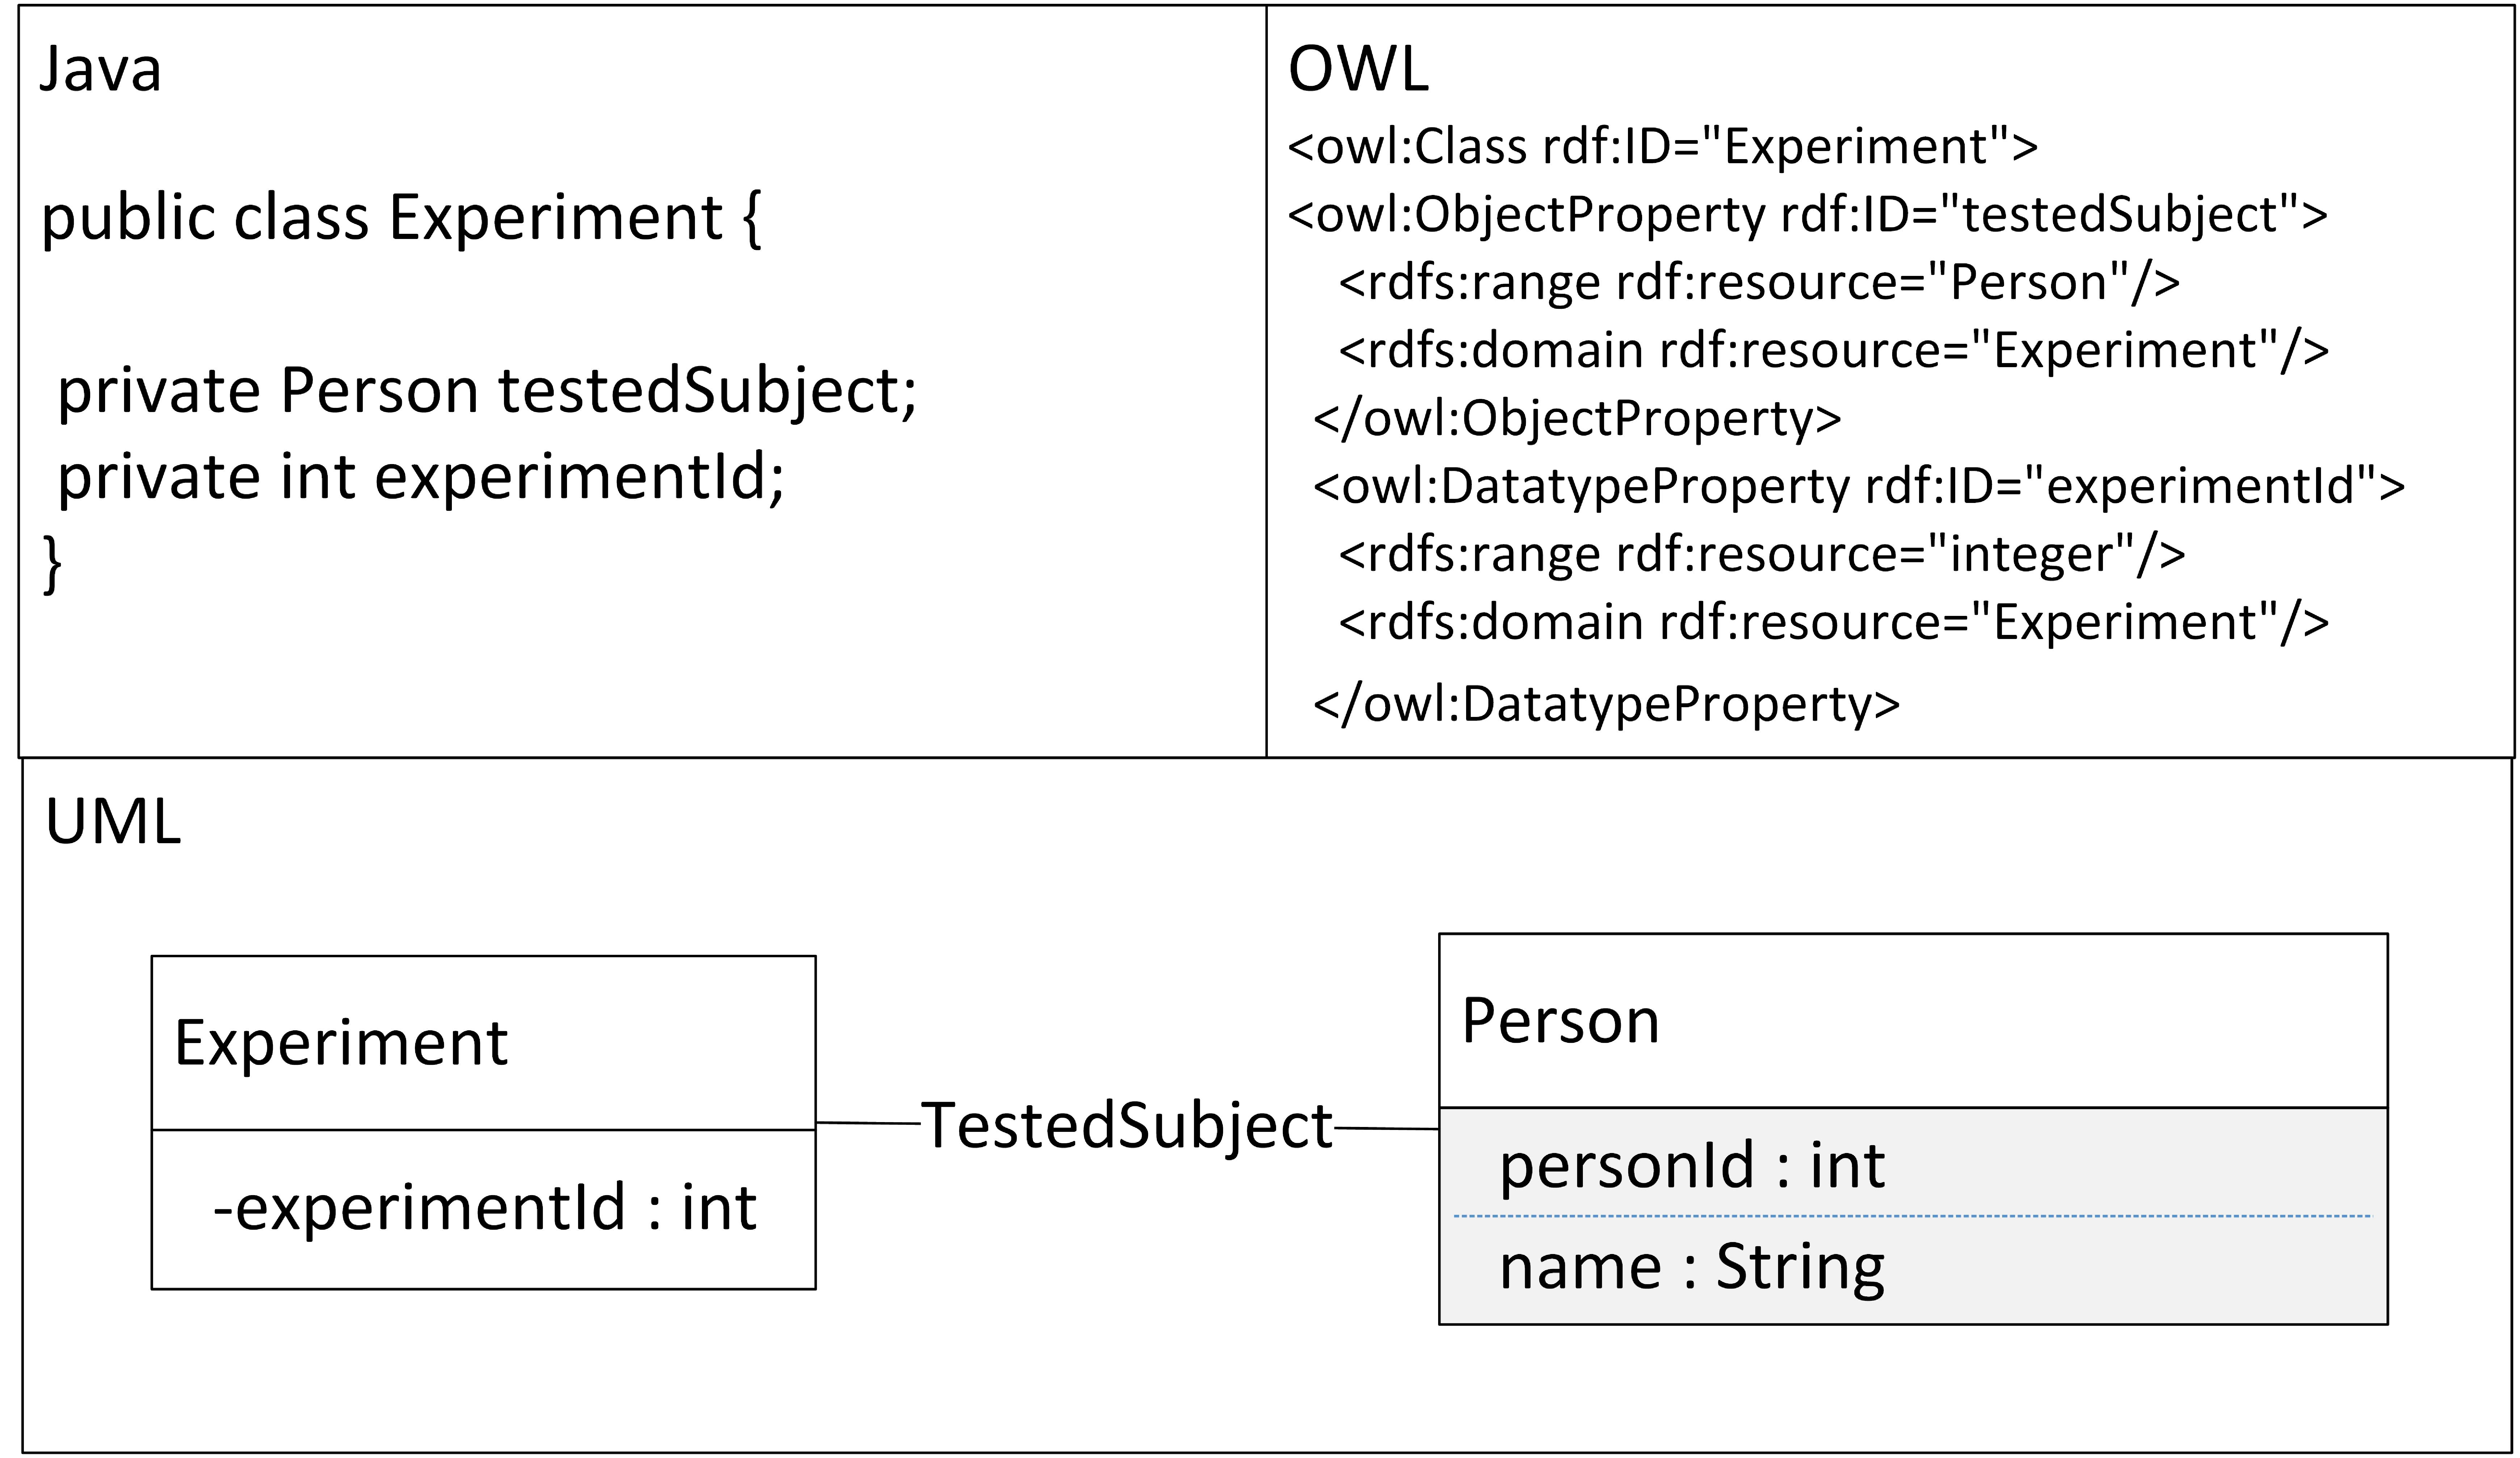
\includegraphics[width = 4.0in]{umlowl1}} \\
\subfloat[Definitions of inheritance and enumeration.]{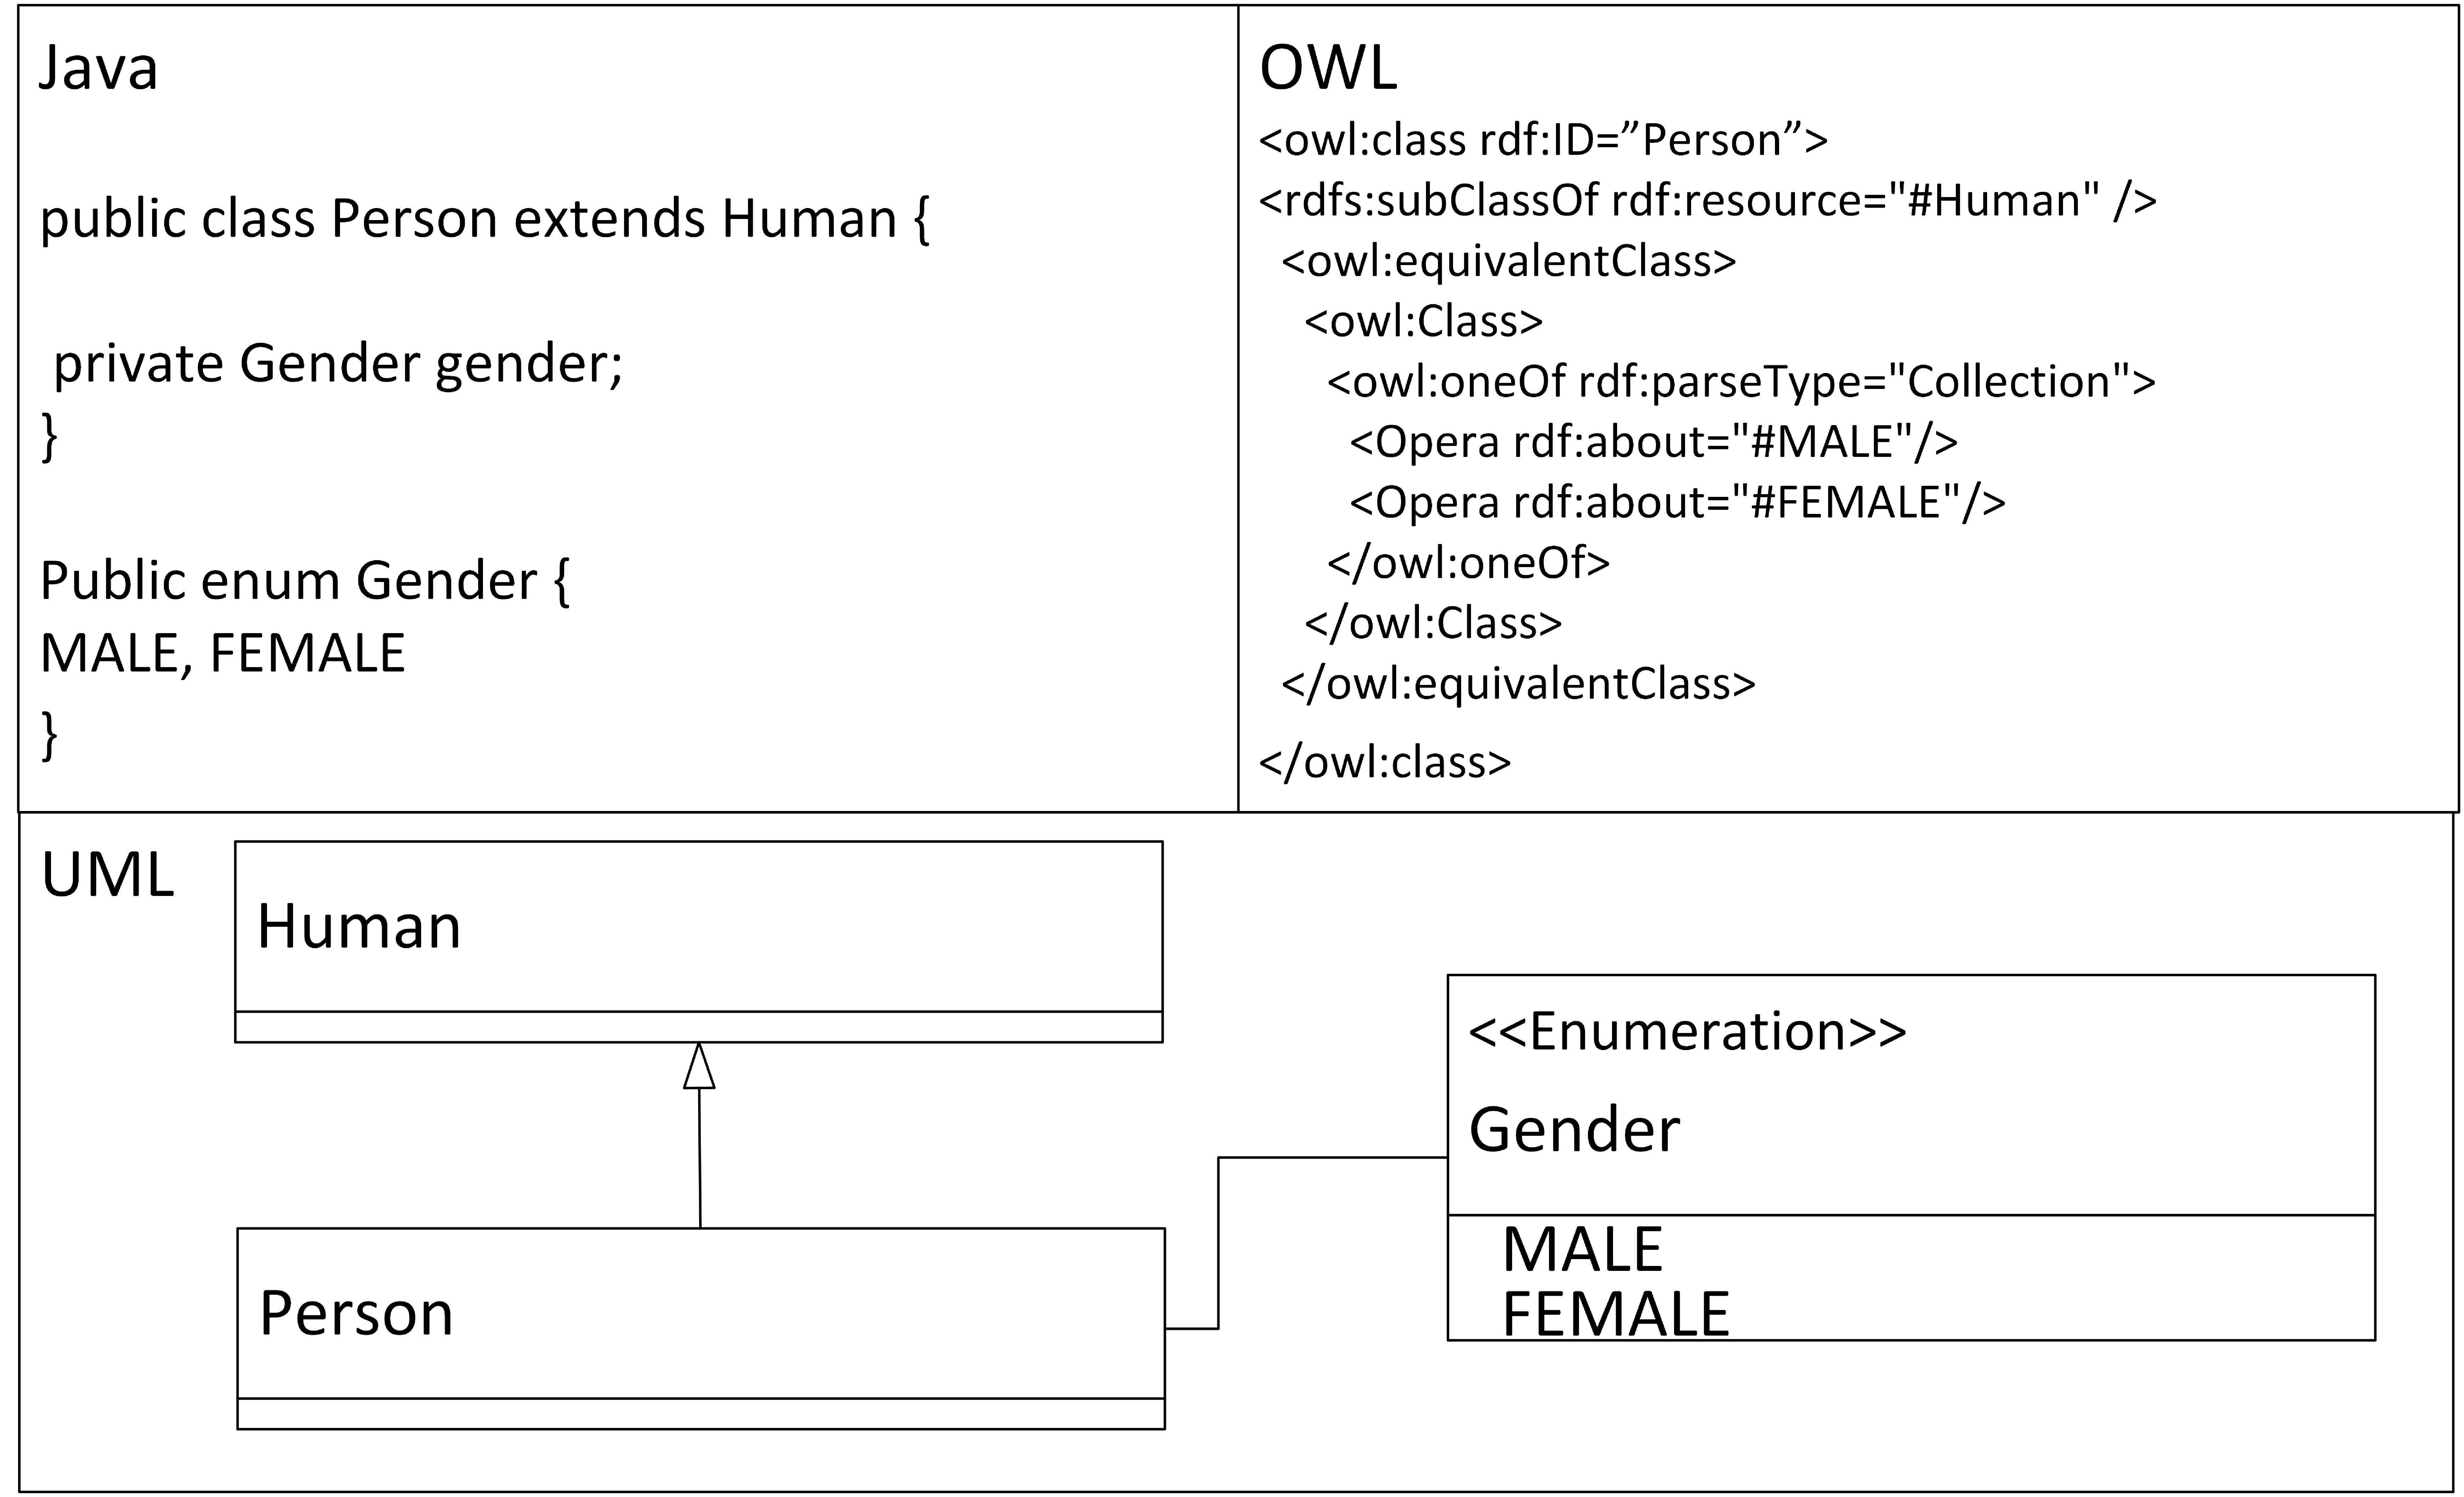
\includegraphics[width = 4.0in]{umlowl2}}  \\
\subfloat[Definitions of disjoint classes.]{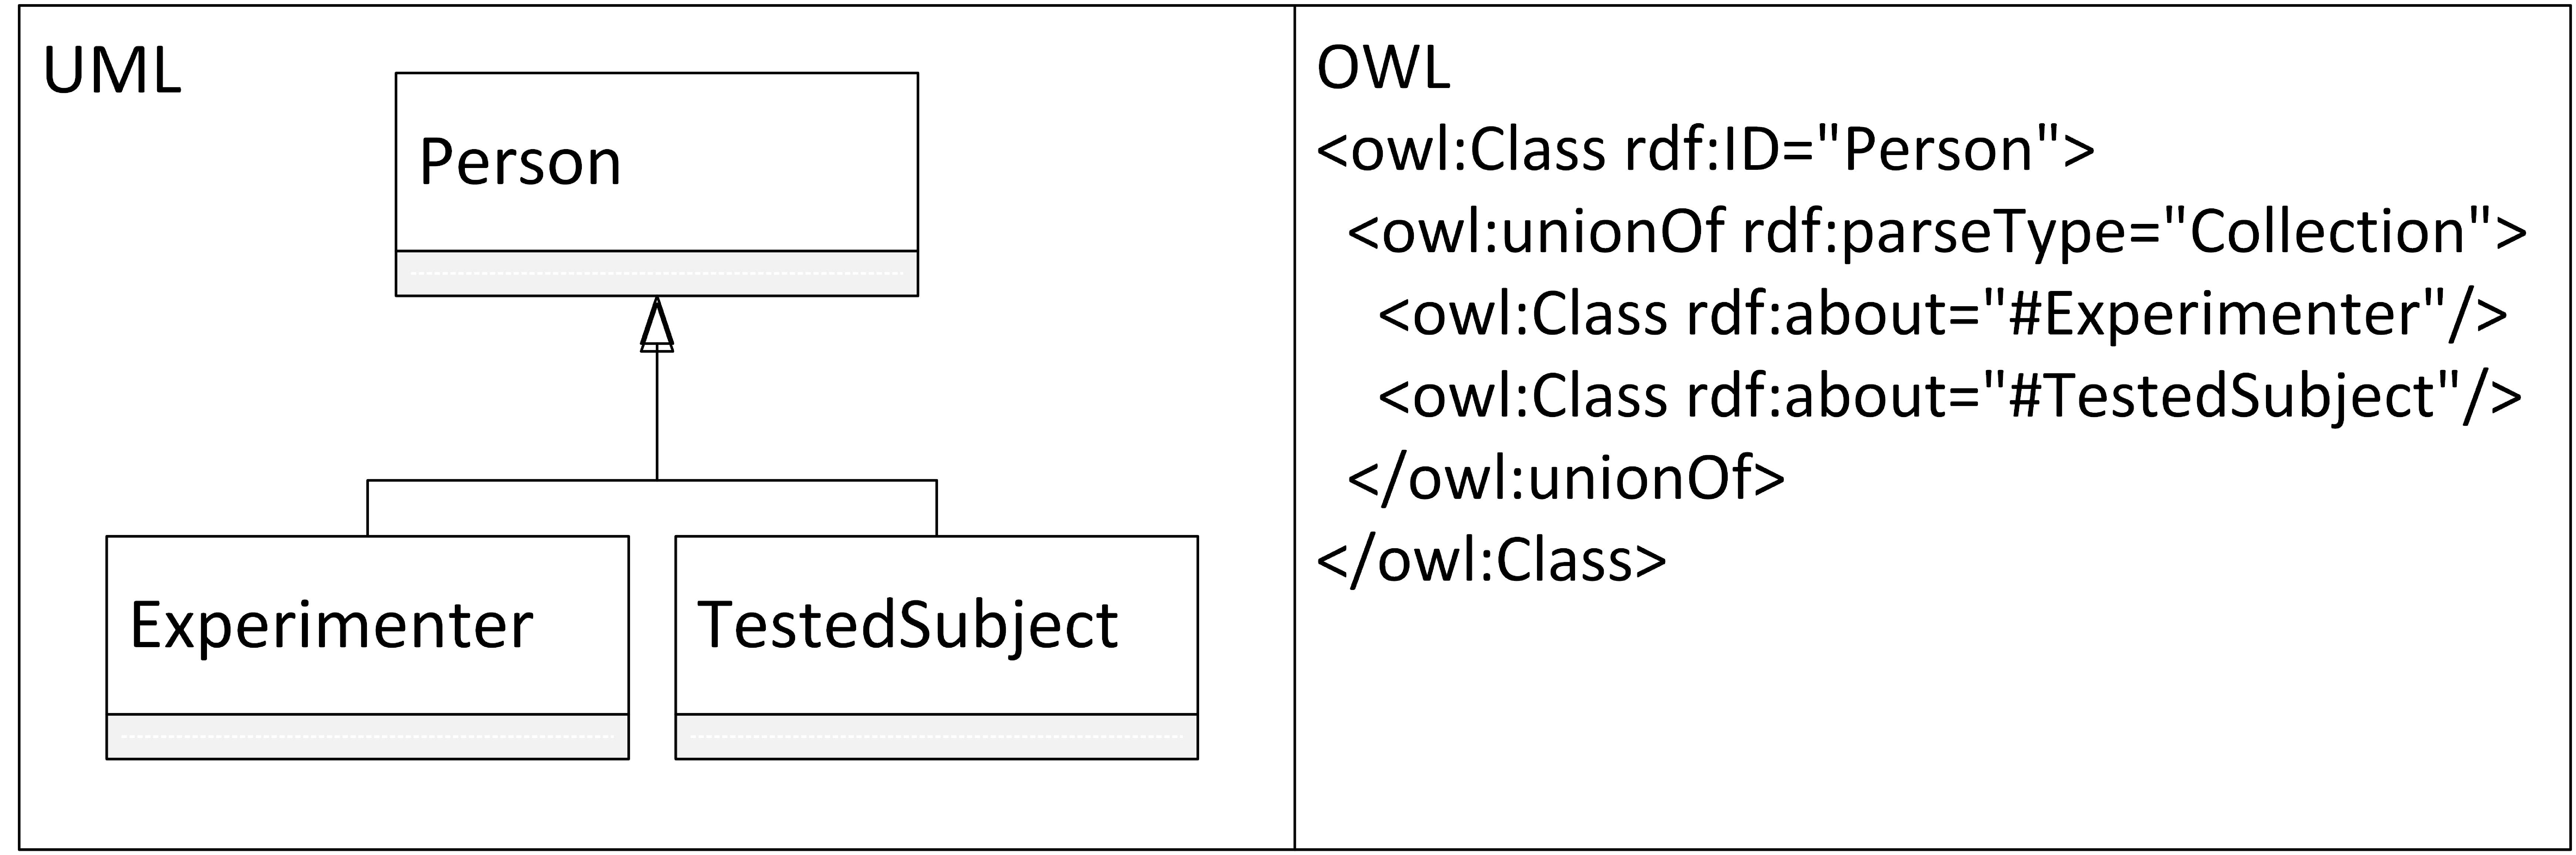
\includegraphics[width = 4.0in]{umlowl3}}
\end{tabular}
% figure caption is below the figure
\caption{Practical examples of Java code, OWL and UML Features.}
\label{fig:umlowlexample}
\end{figure}

\subsection{Related Work}
\label{Related_Work}

Focusing on conventional data sources, specifically a relational database, and an object oriented code, we briefly describe several approaches and tools that map a relational schema or an object-oriented code to the Semantic Web languages. Some of these approaches exist only as initial proposals or prototypes described in scientific papers, while some of them have been really implemented as available frameworks.

A familiar representation of an RDF fact might be represented as a row in a table in a relational database. This table has two columns, corresponding to the subject and the object of the RDF triple. The name of the table corresponds to the predicate of the RDF triple. In this table each row represents a unique instance of the subject. Such a row has to be decomposed for representation as RDF triples \citep{0123820200, 4811327}. The D2RQ~\citep{efeliksik:bizer2004d2rq} is a framework that uses declarative language to describe mappings between relational database schema and RDF. The D2RQ Platform provides possibilities
to query a non-RDF database using the SparQL~\citep{prudhommeaux2008sparql} query language, to access information in a non-RDF database using the Jena API or the Sesame API~\citep{sryll:conf/iswc02/sesame}. METAMorphoses~\citep{svihla} is a data transformation processor from RDB into RDF that uses the mapping described in the template XML document. The XML template defines a set of mapping rules and queries for obtaining data stored in a relational database.

There are approaches and tools that provide limited possibilities to map common syntaxes of an object-oriented code to an OWL representation. These tools map fundamental OWL features (only the basic semantic expressivity of OWL is used).

The mapping of OWL classes to Java Interfaces is described in \citep{sryll:conf/seke04/owl-mapping}. Mapping a Java Interface instead of a common Java class enables the expression of the multiple inheritance of OWL properties. Back transformation is described in \citep{Koide_owlvs.}, where the OWL processor SWCLOS3, which is at the top of the Common Lisp Object System (CLOS), is described. Whereas CLOS allows lisp programmers to develop Object-Oriented systems, SWCLOSS allows programmers to construct domain and task ontologies in software application fields. Java2OWL-S~\citep{DBLP:conf/ic3k/Ohlbach12} is a tool which is able to generate OWL directly. It uses two transformations. The first transformation is from JavaBeans into WSDL (Web Service Description Language). The input of this transformation is formed by a Java class and the output is a temporary WSDL file. The second transformation generates OWL from the WSDL file.

Concerning one-side transformations, these tools with common semantic expressivity work quite satisfactorily because the object-oriented code has poorer semantics than the OWL language. However, in these tools, no possibility to enrich the object-oriented code with missing semantics exists.

The Semantic Object Framework (SOF)~\citep{SOF} utilizes embedded comments in source codes to describe semantic relationships between classes and attributes. The eClass~\citep{Web-Information-Representation} is a solution that changes Java syntax to embed semantic descriptions into the source code. These frameworks enrich the input object-oriented code by missing semantics using either embedded comments or changing the JavaBean syntax. However, the usa of such tools is difficult because it requires a modified compiler and Java interpreter.

\subsection{Semantic Framework}
\label{Semantic Framework}

Drawbacks and limits of the tested frameworks motivated us to introduce a software prototype that enables to add additional semantics into the Java object-oriented code that processes conventional data repositories. A mapping that enables transformation of this code into the Semantic Web language OWL was proposed and implemented as a library - the Semantic Framework presented in Section~\ref{Semantic_Framework}. This approach does not burdensome users with additional demands on programming environment since we used reflective Java annotations - metadata added to the Java source code and retrieved at run-time. Moreover, this additional semantics need not to be written by the programmer directly to the code, but it can be collected from non-programmers using a graphic user interface. The presented approach is discussed from performance (Section~\ref{Performance_evaluation}) and usability (Section~\ref{DISCUSSION}) perspectives. It was validated by integration of the Semantic Framework in the EEG/ERP Portal, together with its registration in the Neuroscience Information Framework (NIF).

\section{Materials and Methods}
\label{Materials_and_Methods}

\subsection{Semantic Framework}
\label{Semantic_Framework}

Taken into account differences in semantic expressivity described in Section~\ref{Conventions}, we proposed a custom approach that transforms a common object-oriented syntax to an OWL syntax. This solution is usable by software engineers and not only by experts in the Semantic Web. It serves a community of developers/researchers that develop/use object-oriented systems and need to provide an output in the Semantic Web languages. To support this idea, we decided to use only standard syntactic structures of a commonly used programming language. Java stores data in JavaBeans\footnote{JavaBeans, as reusable components, are named Java classes with class attributes which are accessed only by get/set methods.}, often called Plain Old Java Objects (POJOs). The transformation of JavaBean representation into an OWL ontology is described in Definition~\ref{def:JavaBean structure extraction process}.

\begin{definition}
\label{def:JavaBean structure extraction process}
(Extraction process from a JavaBean structure)

\emph{The process is the transformation of a set of JavaBeans J to an ontology O that satisfies:}

\emph{$\forall$ $J{}_{\text{i}}$ $\exists$ OWL class $OC{}_{\text{i}}$ $\in$ O}.

\emph{$\forall$  $J{}_{\text{j}}$ is a superclass of $J{}_{\text{i}}$ $\exists$ OWL class $OC{}_{\text{j}}$ is a superclass of OWL class $OC{}_{\text{i}}$  $\in$  O}.

\emph{$\forall$ field $\in$ $Jf{}_{\text{i}}$ $\exists$  class $OC{}_{\text{i}}$ $\in$  O; its extent is a DataType property $\in$  O $\Leftrightarrow$ $Jf{}_{\text{i}}$ extent is an atomic type}.

\emph{$\forall$ field $\in$ $Jf{}_{\text{i}}$ $\exists$  class $OC{}_{\text{i}}$ $\in$ O; its extent is an Object property $\Leftrightarrow$ $Jf{}_{\text{i}}$ extent is a class $\in$ $J{}_{\text{i}}$}.

\emph{$\forall$ instance of  $J{}_{\text{i}}$ $\bigwedge$ $\forall$ field $Jf{}_{\text{ij}}$  $\exists$ OWL literal $OL{}_{\text{ij}}$ $\in$ O $\hat{=}$ field $\in$ $Jf{}_{\text{ij}}$}.

\end{definition}

%\subsubsection{Proposed Mapping}
%\label{Proposed_Mapping}

An example of a mapping of a Java class to an OWL construct is shown in Listing~\ref{Java_class_property_Definition}. The Java class \emph{Experiment} has two attributes, \emph{testedSubject} and \emph{experimentId}. The first one is an association relation to the \emph{Person} class, while the second one is an atomic type. Get/set methods are omitted to keep readability. Listing \ref{OWL_individual_Instance} shows a fundamental serialization of this class into an OWL structure. When a sample instance of a described class with assigned sample values \emph{testedSubject=John Smith} and \emph{experimentId=21} is created, its representation is transformed to an \emph{OWL individual}. The serialization of \emph{DataTypeProperty} is straightforward, the property value is directly serialized. The serialization of \emph{ObjectProperty} is solved by serializing an object id value or by placing a link that points to the data in the case of binary files.

\begin{lstlisting}[label=Java_class_property_Definition,caption=Java Class]
package cz.zcu.kiv;

public class Experiment {

 private Person testedSubject;
 private int experimentId;
}

\end{lstlisting}

\begin{lstlisting}[label=OWL_individual_Instance,caption=OWL Individual Instance]

<cz.zcu.kiv:Experiment rdf:about=
  "http://cz.zcu.kiv#Experiment_21">
  <cz.zcu.kiv:testedSubject>
    <cz.zcu.kiv:Person rdf:about=
      "http://cz.zcu.kiv#Person_511991">
      <cz.zcu.kiv:name rdf:datatype=
        "http://www.w3.org/2001/XMLSchema#string">
        John Smith
      </j.1:name>
    </cz.zcu.kiv:Person>
  </cz.zcu.kiv:testedSubject>
  <cz.zcu.kiv:experimentId rdf:datatype=
    "http://www.w3.org/2001/XMLSchema#int">
    21
  </cz.zcu.kiv:experimentId>
</cz.zcu.kiv:Experiment>
\end{lstlisting}

Although the described mapping works quite satisfactorily, different concepts described in Section~\ref{Conventions} are not covered. When we want to use more capabilities of OWL, we have to enrich the object-oriented code with missing semantics. Looking for a suitable way to extend a current object-oriented code, we decided to extend a proposed preliminary idea~\citep{conf/iceis/JezekM11} based on using Java Annotations~\citep{JavaTutorialAnnotations}.

Java Annotations have several benefits. Firstly, they can be added, as a special form of syntactic metadata, to a Java source code. Secondly, they are reflective, i. e. they can be embedded within the compiled code and retrieved at runtime. Thus, we can directly execute a compiled code in the transformation input. Moreover, Java Annotations are a part of the Standard Java Development Kit; they can be processed immediately using Java 5.0 or higher. Finally, Java Annotations are used in current software development (by several common frameworks, e.g. Spring, Hibernate, Java Persistent API); hence, software developers can work with this extension without difficulties.

The theoretical extraction of JavaBeans annotations and their transformations to OWL documents is formally described in Definition~\ref{def:Java_annotation_extraction_process}.

\begin{definition}
\label{def:Java_annotation_extraction_process}
(Java annotation extraction process)

\emph{The process is the transformation of a set of Java annotations JA to a resources R  in the ontology O that satisfies:}

\emph{$\forall$ $JA{}_{\text{i}}$ $\exists$ OWL class $R{}_{\text{i}}$ $\in$ O $\Rightarrow$ $JA{}_{\text{i}}$ $\in$ a class annotation}.

\emph{$\forall$ $JA{}_{\text{i}}$ $\exists$ OWL property $R{}_{\text{i}}$ $\in$ O $\Rightarrow$ $JA{}_{\text{i}}$ $\in$ a property annotation}.

\end{definition}

An example of using two annotations is given in Listing~\ref{Annotated_Java_Bean_Example}. The class Person has an attribute testedPerson as defined in Listing~\ref{Java_class_property_Definition}. The first annotation defines an~\emph{equivalent class} to the Experiment class. The second annotation shows the definition of an \emph{equivalent property} of the testedSubject property. The serialization of this JavaBean is shown in Listing~\ref{Annotated_Java_Bean_OWL_Serialization}.

\begin{lstlisting}[label=Annotated_Java_Bean_Example,caption=Annotated Java Bean Example]
package cz.zcu.kiv;

@EquivalentClass
  ("http://cz.zcu.kiv/Measurement")
public class Experiment {

  @EquivalentProperty
    ("http://cz.zcu.kiv/TestedSubject")
  private Person testedPerson;
}
\end{lstlisting}


\begin{lstlisting}[label=Annotated_Java_Bean_OWL_Serialization,caption=Annotated Java Bean OWL Serialization, escapechar=@]
<owl:Class rdf:about=
  "http://cz.zcu.kiv/Measurement"/>
<owl:Class rdf:about=
  "http://cz.zcu.kiv#Experiment">
 @\textbf{
 $<$owl:equivalentClass rdf:resource= }@
 @\textbf{    "http://cz.zcu.kiv/Measurement"/$>$
    }@
</owl:Clas>
<owl:ObjectProperty rdf:about=
  "http://cz.zcu.kiv#testedPerson">
@\textbf{
  $<$owl:equivalentProperty rdf:resource=  }@
@\textbf{    "http://cz.zcu.kiv/TestedSubject"/$>$
  }@
  <rdfs:domain rdf:resource=
   "http://cz.zcu.kiv#Experiment"/>
</owl:ObjectProperty>
\end{lstlisting}

We selected the concepts that have a~class and/or property extent~\citep{BMEI_jezek_moucek} and defined a~set of annotations with their mapping to corresponding OWL constructs (Table \ref{tab:Java annotations to OWL mapping}. Most of the proposed annotations are parameterizable; parameter values shown in Table~\ref{tab:Java annotations to OWL mapping} are examples; they can be changed according to the needs of a specific domain.

\begin{table}

\centering
\footnotesize
\renewcommand{\arraystretch}{1}
\tabcolsep=0.11cm
\catcode`\-=12
\caption{\label{tab:Java annotations to OWL mapping}OWL Mapping of Java Annotations}
\begin{tabular}{ll}

\hline
\textbf{Java Annotation} & \textbf{OWL construct}
\tabularnewline
\hline
@EquivalentClass & $<$owl:equivalentClass rdf:resource=\\
("http://www.kiv.zcu.cz/Person") & \hspace{3mm}"http://www.kiv.zcu.cz/Person"/$>$
\tabularnewline
\hline
@EquivalentProperty & $<$owl:equivalentProperty rdf:resource=\\
("http://www.kiv.zcu.cz/first\_name") &\hspace{3mm}"http://www.kiv.zcu.cz/first\_name"/$>$ \\

\hline
@Symmetric & $<$rdf:type rdf:resource="http:/www.w3.org\\
& /2002/07/owl\#SymmetricProperty"/$>$ \\
\hline
@Inverse & $<$owl:inverseOf rdf:resource=\\
("http://www.kiv.zcu.cz/givenname") &\hspace{3mm}"http://www.kiv.zcu.cz/givenname"/$>$\\

\hline
@AllValuesFrom & $<$owl:allValuesFrom rdf:resource=\\
("http://www.kiv.zcu.cz/\#Persons") &\hspace{3mm}"http://www.kiv.zcu.cz/\#Persons"/$>$ \\
\hline
@Transitive& $<$rdf:type rdf:resource=\\
 &\hspace{3mm}"http://www.w3.org/2002/07/owl\\
& \#TransitiveProperty"/$>$ \\
\hline
@AllDifferent & $<$rdf:type rdf:resource=\\
("http://www.kiv.zcu/Experiment") & \hspace{3mm}"http://www.kiv.zcu.cz/\#AllDifferent"/$>$\\
\hline
@DifferentFrom & $<$owl:differentFrom rdf:resource=\\
("http://www.kiv.zcu.cz/Experiment") & \hspace{3mm}"http://www.kiv.zcu/Experiment"/$>$ \\
\hline
@SameAs & $<$owl:sameAs rdf:resource=\\
("http://www.kiv.zcu.cz/Experiment") & \hspace{3mm}"http://www.kiv.zcu/Experiment"/$>$ \\
\hline
@Cardinality(1) &         $<$owl:cardinality rdf:datatype=\\
&\hspace{3mm}"http://www.w3.org/2001/XMLSchema\\
&\hspace{3mm}\#int"$>$1$<$/owl:cardinality$>$\\
\hline
@MaxCardinality(1) & $<$owl:maxCardinality rdf:datatype\\
&\hspace{3mm}="http://www.w3.org/2001/XMLSchema\\
&\hspace{3mm}\#int"$>$1$<$/owl:maxCardinality$>$\\

\hline
@MinCardinality(1) & $<$owl:minCardinality rdf:datatype\\
&\hspace{3mm}="http://www.w3.org/2001/XMLSchema\\
&\hspace{3mm}\#int"$>$1$<$/owl:minCardinality$>$\\

\hline
@SomeValuesFrom & $<$owl:someValuesFrom rdf:resource=\\
 ("http://www.kiv.zcu/Person") & \hspace{3mm} "http://www.kiv.zcu/Person"/$>$\\
\hline

\end{tabular}


\end{table}

%\subsubsection{Implementation}
%\label{Implementation}

The described mapping was implemented as a library named the Semantic Framework\footnote{The project repository is available at: https://github.com/NEUROINFORMATICS-GROUP-FAV-KIV-ZCU/Semantic-Framework}. It processes a~set of JavaBeans as an input and produces an ontology document as an output. We did not implement the Semantic Framework from scratch, but extended and integrated already existing tools. The core of the system is extended JenaBean~\citep{citeulike:JenaBean} that internally uses the Jena Framework~\citep{morningboat:jena16} to persist JavanBeans. Figure~\ref{fig:Semantic_Framework} shows the component diagram of the Semantic Framework. The first subcomponent is the extended JenaBean that reads and parses JavaBeans and related Java annotations. The output of the \emph{Extended JenaBean} component is an internal JenaBean model that is transferred to the second, \emph{Ontology Model Creator}, subcomponent. This subcomponent creates an ontology model using an \emph{Ontology Model Factory} and Jena API methods. This ontology model extends access to the statements in a RDF data collection by adding support for constructs that are expected to be in an ontology. However, all of the state information is still encoded as RDF triples and stored in the RDF model. The resulting ontology model (in the form of an ontology document) is further processed by the last subcomponent, \emph{OWL API}~\citep{DBLP:journals/semweb/HorridgeB11}, which provides the ontology model into a selected serialization format. The UML diagram describing the usage of the Semantic Framework is available in Figure~\ref{fig:Semantic_Framework_class_diagram}.

\begin{figure}
% Use the relevant command to insert your figure file.
% For example, with the graphicx package use
  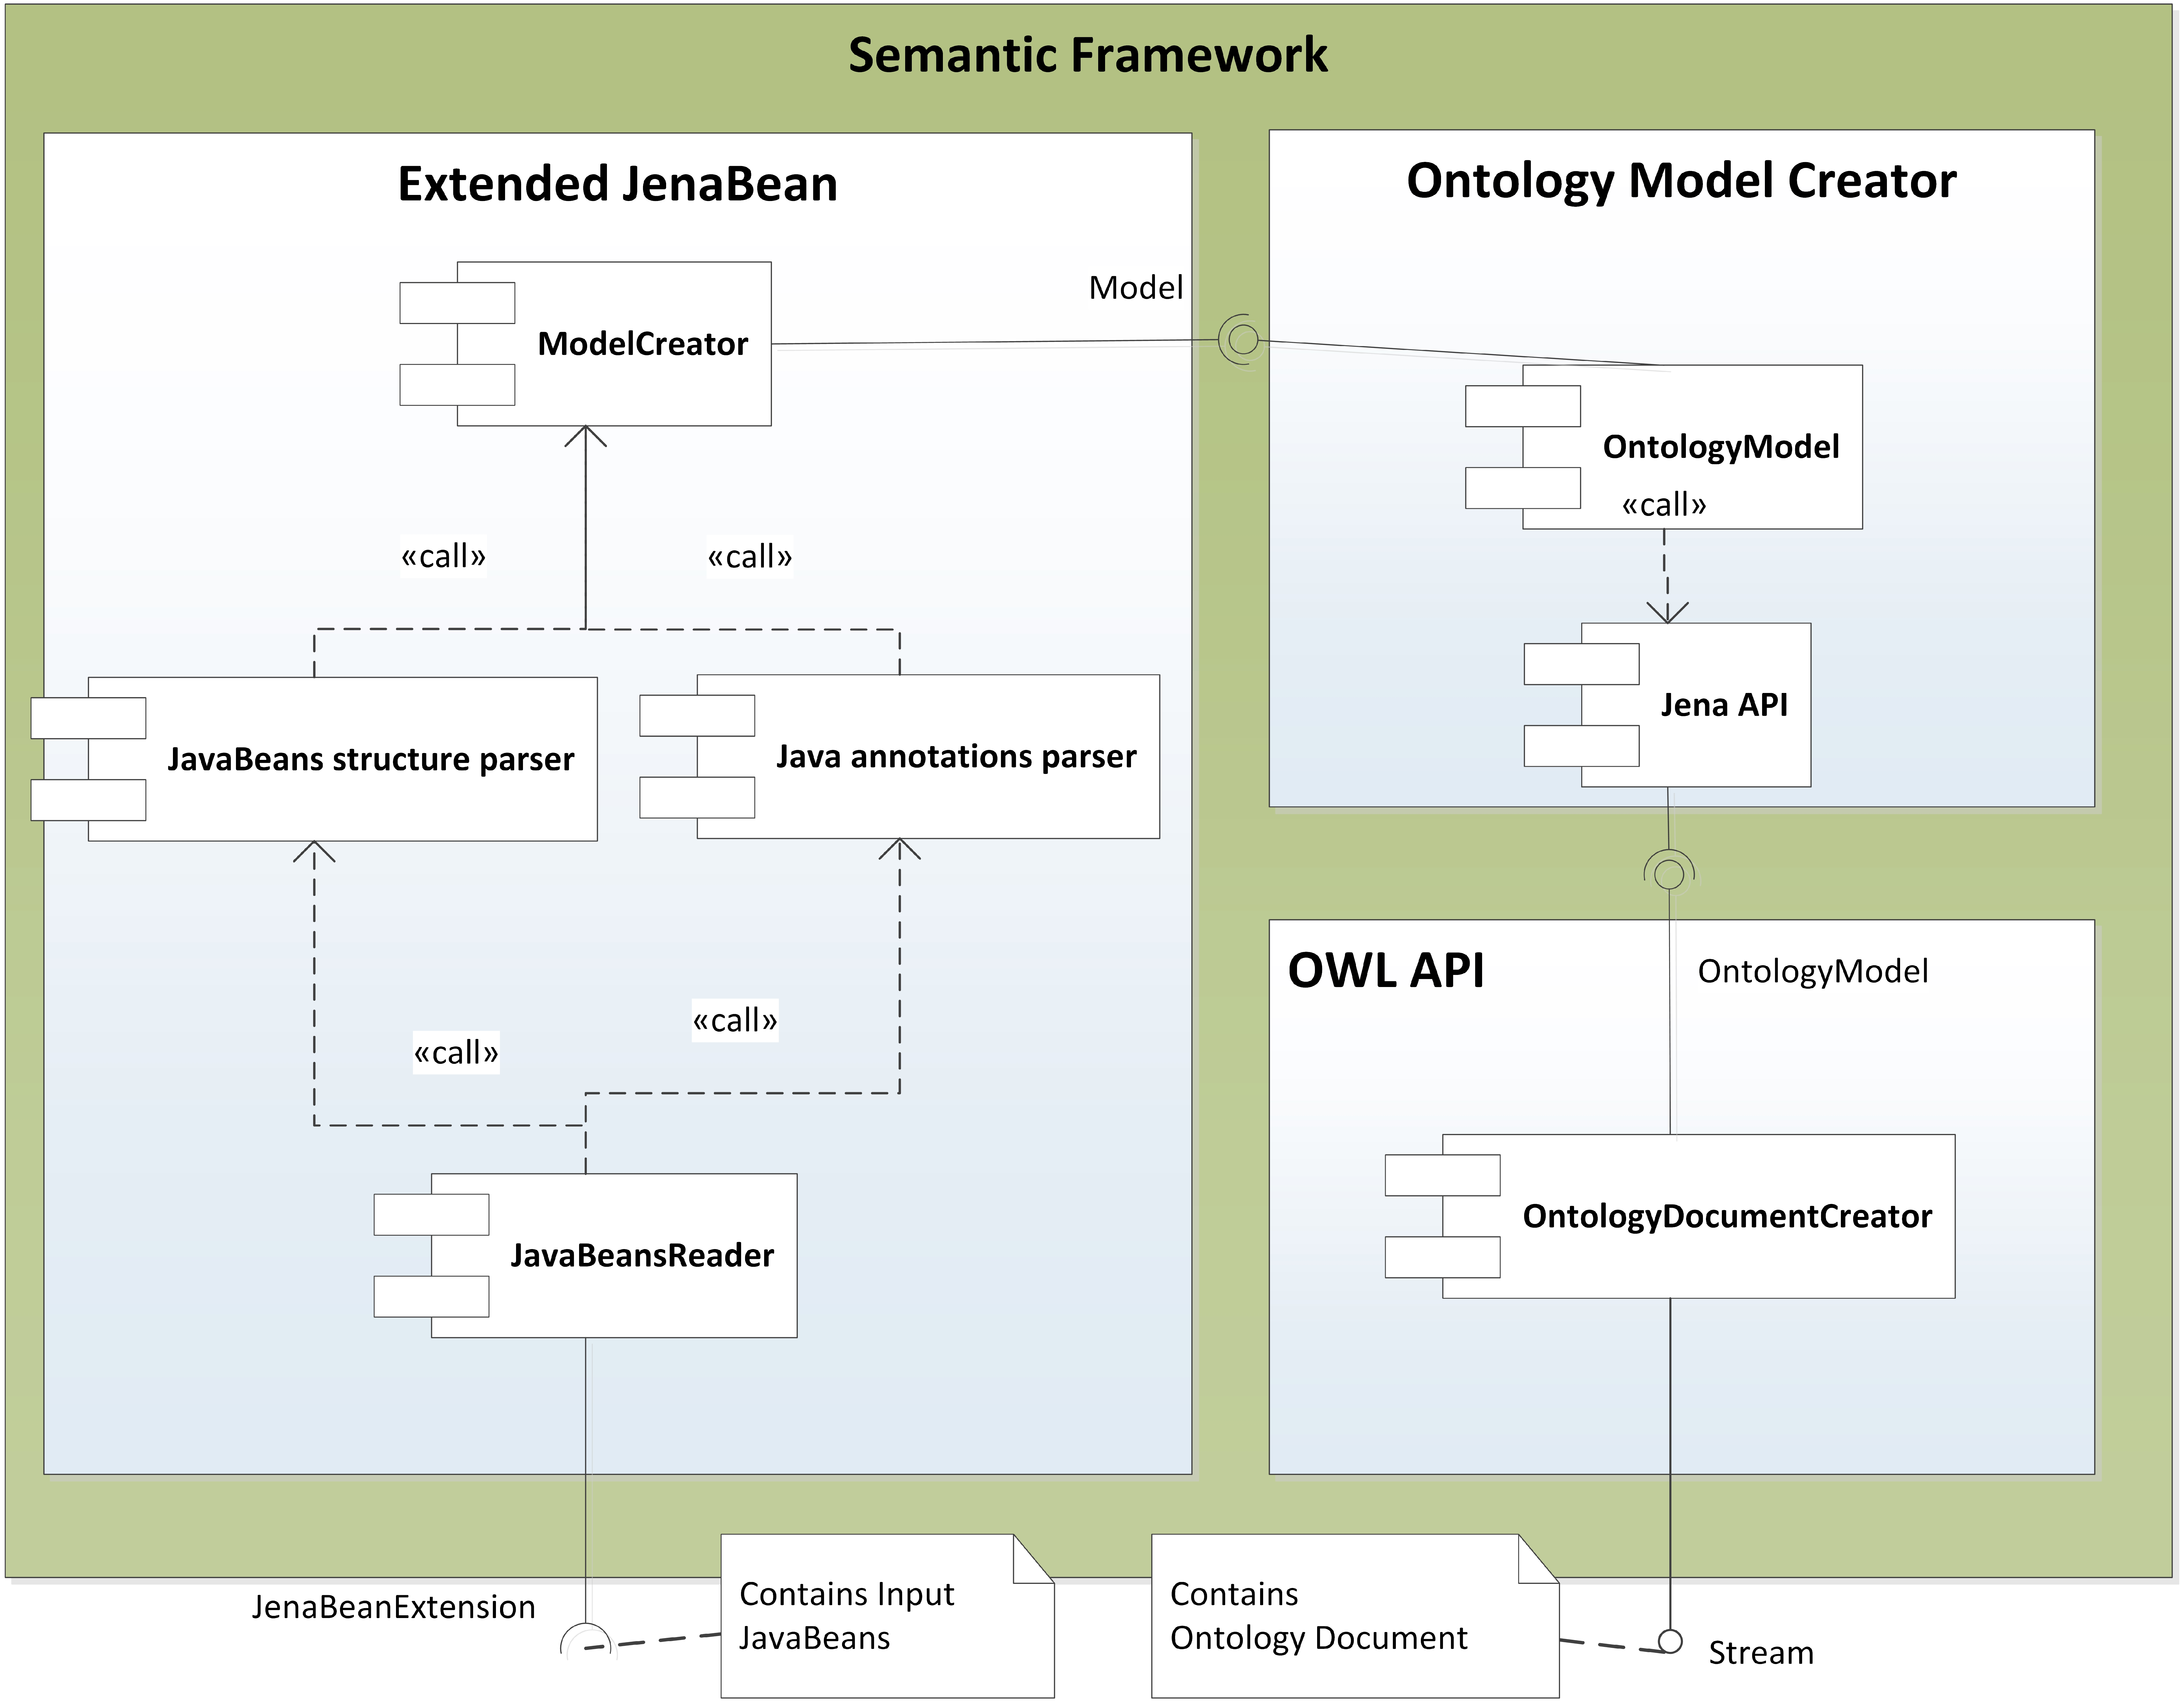
\includegraphics[width=15cm]{SemanticFramework_Component_Model}
% figure caption is below the figure
\caption{Component Diagram of the Semantic Framework. The Semantic Framework reads a list of input JavaBeans using an implemented reader based on Java Reflection API \citep{jlfalcone:sun:06}. This list passes through two parsers. The first one reads a JavaBean structure; the second one reads supplemented annotations. The parsers create an internal JenaBean representation. This representation is read by Jena API, which provides an ontology model processed by an OWL API. The OWL API implements existing OWL syntaxes and provides methods for serializing the ontology model.}
\label{fig:Semantic_Framework}
\end{figure}


\begin{figure}
\center
% Use the relevant command to insert your figure file.
% For example, with the graphicx package use
  
\includegraphics[width=15cm]{SemanticFramework_uml}
% figure caption is below the figure
\caption{Class Diagram of the Semantic Framework Interface. Actor1 represents a client program. The client uses the interface \emph{JenaBeanExtension} having the method \emph{getOntologyDocument} that returns an ontology document in a~stream. The returned stream can be serialized into supported formats by an \emph{OwlApi} interface calling the \emph{convertToSemanticStandard} method.}
\label{fig:Semantic_Framework_class_diagram}
\end{figure}


\section{Results}
\label{Results}

\subsection{Performance Evaluation}
\label{Performance_evaluation}

%\subsubsection{Experimental Verification}
%\label{Experimental_Verification}

The time complexity of the Semantic Framework was tested in the following way. Firstly, we prepared a set of instances of the class \emph{Experiment}. Then, we assigned instances of the classes \emph{Person}, \emph{Scenario}, \emph{Hardware} and \emph{Data} to each experiment. The class \emph{Person} was extended by the set of supported annotations from Table~\ref{tab:Java annotations to OWL mapping}. The performance tests were run ten times and the result was calculated as an average of all program runs. The time complexity of the transformational process is linear with respect to the number of instances. The tested syntaxes are functionally equivalent; they differ only in the format of the serialized output document~\citep{Wurlitzer:Beckett:04:RSS}.

%\begin{figure}
  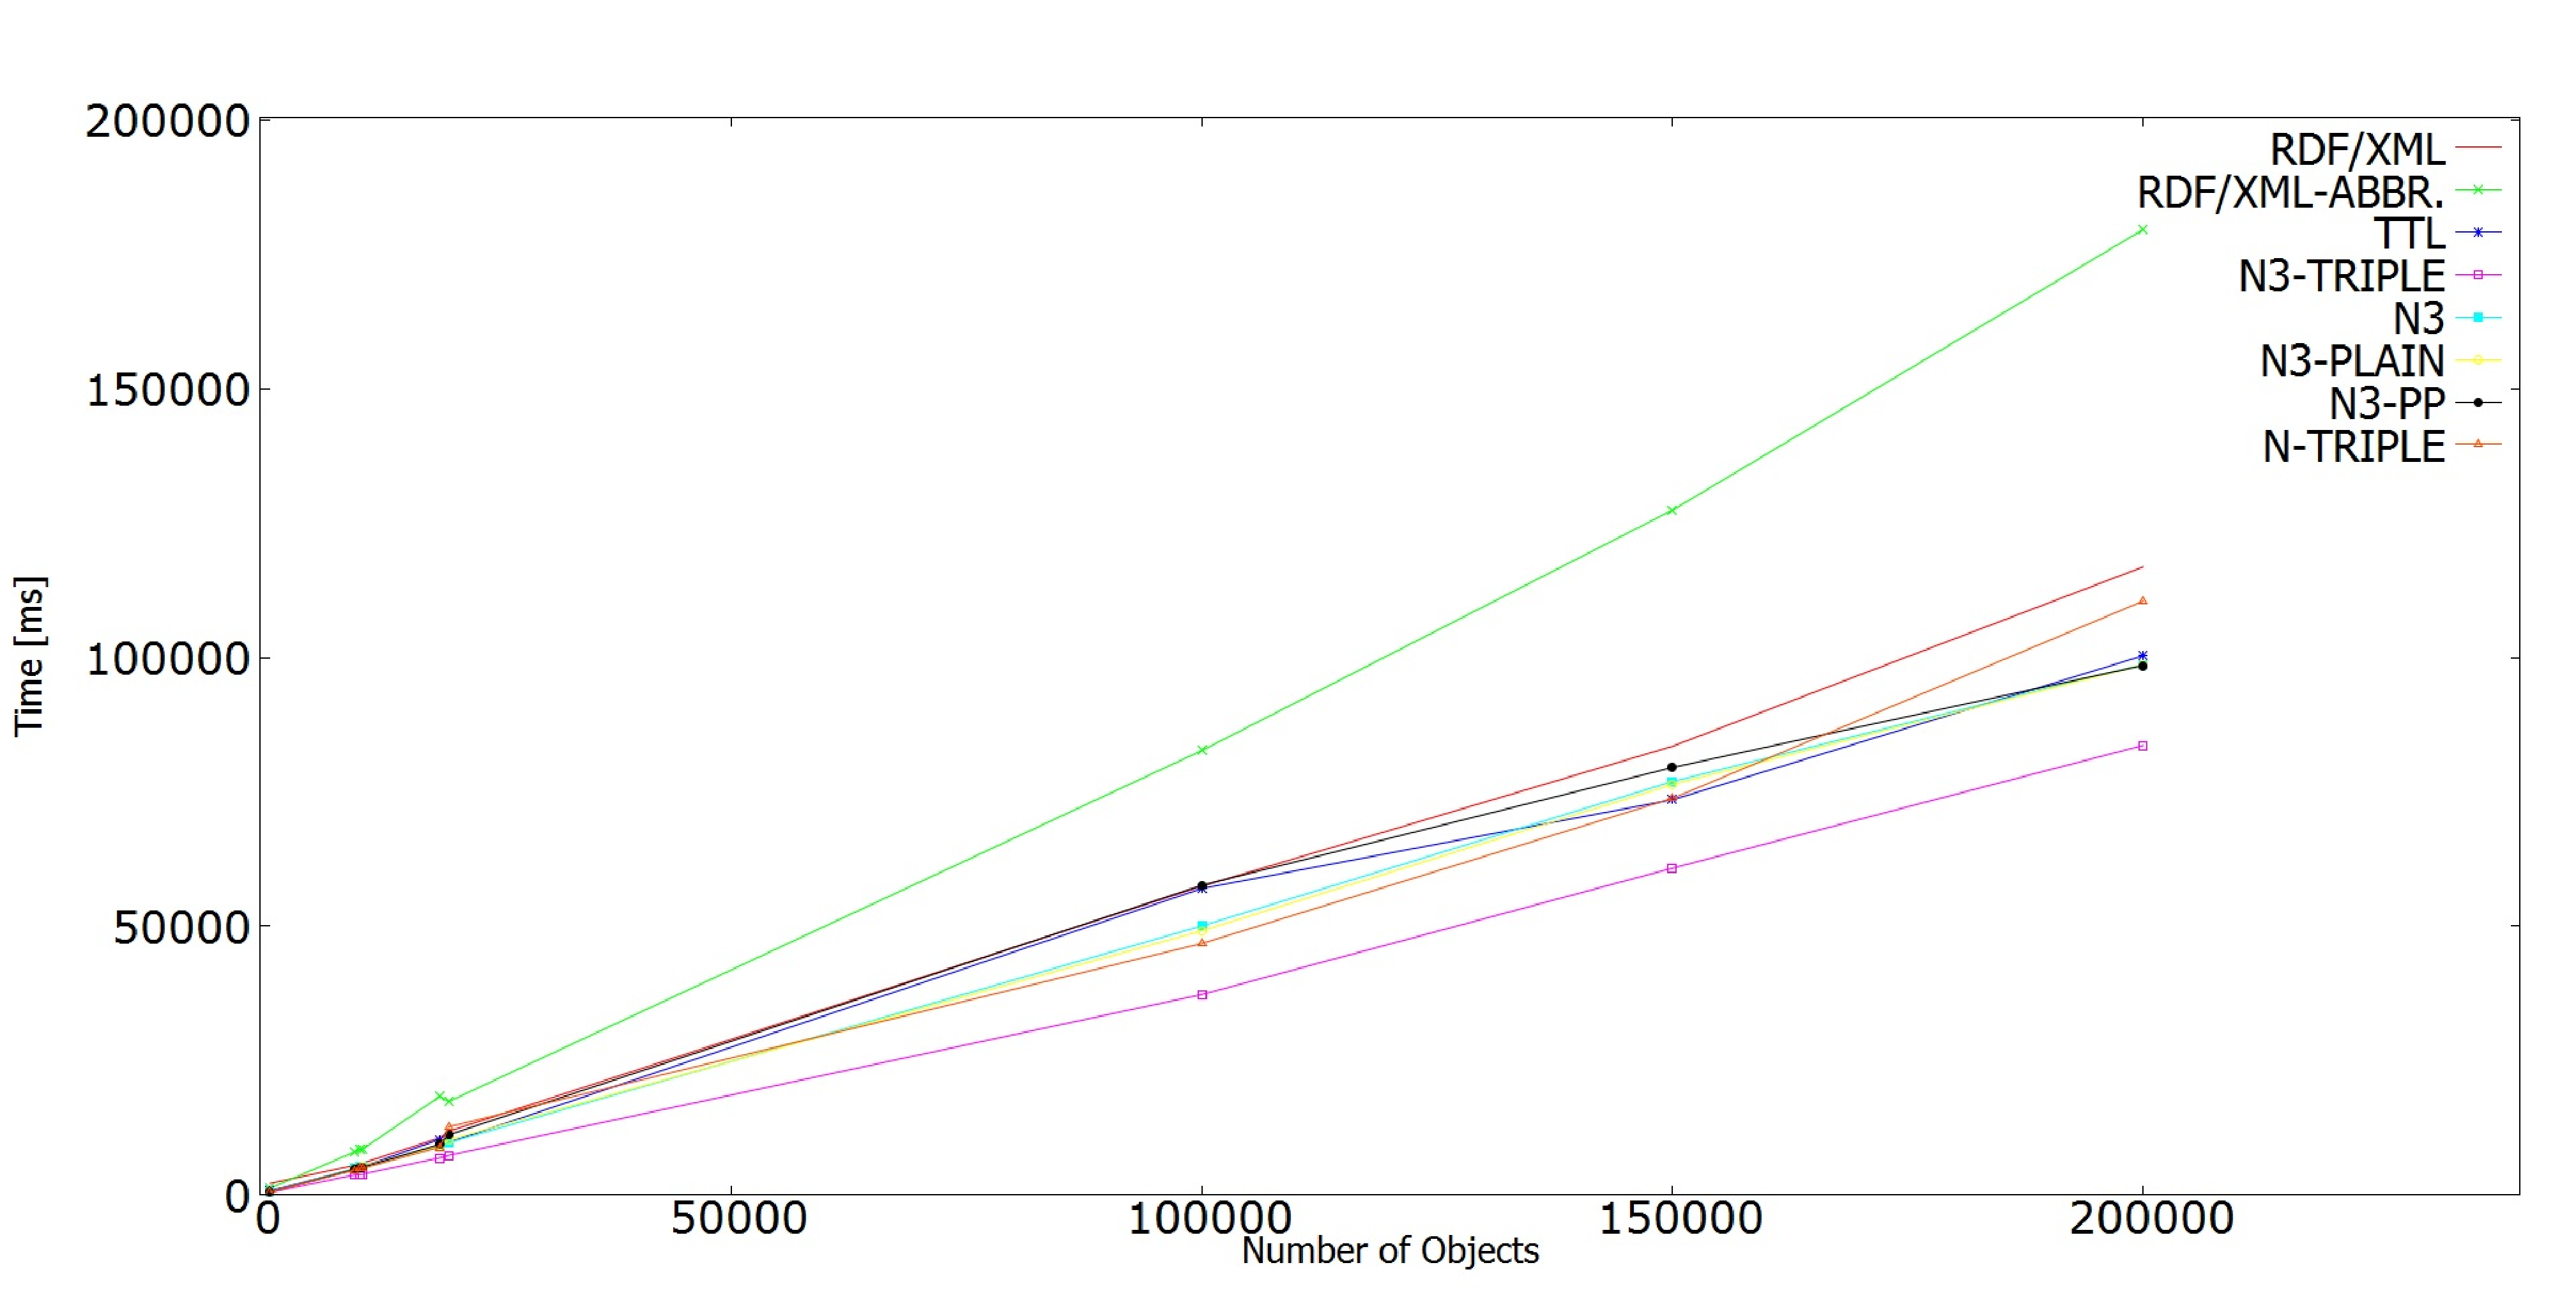
\includegraphics[width=18cm]{result}
% figure caption is below the figure
%\caption{Time complexity of the transformation with respect to the number of objects for supported syntaxes. The time complexity is fundamentally linear for each syntax, the transformation process is directly dependent only on the number of input objects.}
%\label{fig:results}
%\end{figure}

\subsection{Experimental Evaluation}
\label{experimental_evaluation}

%\subsubsection{Experimental Ontology}
%\label{Experimental_Ontology}

We defined a simple ontology that describes the experimental work in our laboratory. Semantically, it is a~modified subset of the NEMO ontology with added terms describing an experimental protocol and restrictions during an experimental session. The ontology structure corresponds to metadata collected during experiments. These metadata are divided into several semantic groups:

\begin{itemize}
\item Activity - describes a predefined experimental protocol. It includes information about audio and/or video stimulation, instructions given to tested subjects, detailed descriptions of stimuli (target vs. non-target, timing), etc.
\item Environment - describes surrounding conditions such as weather, daytime or room temperature.
\item Tested subject - includes information about the tested subject such as laterality, education, age, gender, diseases, and disability.
\item Hardware equipment - describes e.g. the type, producer and serial number of the hardware used.
\item Software equipment - describes software used during the experiment. It includes e.g. the name of the software, the version and the producer, and configuration files if they are used.
\item Used electrodes - describes the type, impedance, location, the system used and fixation of the electrodes.
\item Data digitalization - describes a set of parameters that influence conversion of data using a specific analogue-digital converter. It includes filtration, sampling frequency, and band-pass.
\item Signal analysis - describes basic analytic steps during the EEG/ERP signal processing. It includes the determination of the length of the pre- and post-stimulus part of the signal, the number of epochs, and the verbal description of the signal-processing procedure.
\item Data presentation - describes experimental results or assumptions needed to reproduce an experiment. It includes averaged ERP waves (images of averaged waves), grand averages (images of grand averages), evolution of the ERP signal in time and space (images showing the ERP signal propagation over the scalp), waves description (description of well-known or new waves formed during the study), and the link to all raw experimental data.
\item Signal artifact - contains information describing a compensation method that prevents formation of artifacts. When a method for removing artifacts is used, its description is also placed there. When some artifact totally degrades the signal, the experimenter can define conditions when it is possible to assume that the signal is totally useless.
\end{itemize}

This ontology was built within the development of the EEG/ERP Portal~\citep{ISI:000306821100004}, a~web application for the storage, long-term management and sharing of electrophysiology data. The data layer of the Portal is implemented using a relational database (Oracle 11g) and POJOs. An object-relational mapping (ORM) is ensured by the Hibernate framework~\citep{Bauer:2006:JPH:1212283}. The internal structure (classes and their relationships, annotations) of the data layer is implemented according to the defined ontology. The application layer was developed using the Spring Framework; the presentation layer uses Apache Wicket. Upload of data and metadata is ensured via a set of predefined web forms.

The Semantic Framework was integrated into the EEG/ERP Portal (Figure~\ref{fig:Semantic_Framework_Integration_in_EEG_ERP_Portal}). The internal logic\footnote{Spring MVC is used. It practically implements a Model-View-Controller design pattern.} calls a Semantic Framework API (the UML diagram describing the Semantic module API in the EEG/ERP Portal is shown in Figure~\ref{fig:Semantic_Framework_Integration}) using a built-in timer at regular intervals; the ontology document is stored in a temporary file that is further serialized into a~required syntax. Syntaxes \emph{RDF/XML}, \emph{OWL/XML}, \emph{RDF/XML-ABBREV}, \emph{N-TRIPLE}, \emph{TURTLE}, \emph{N3}, \emph{N3-PP}, \emph{N3-PLAIN}, and \emph{N3-TRIPLE} are currently supported. The \emph{SemanticMultiController} is listening on a specific URL with a \emph{GET} parameter. For instance, when a reasoner visits the URL \emph{http://eegdatabase.kiv.zcu.cz/seman tic/getOntology.html?type=turtle}, it obtains the OWL document in the \emph{turtle} syntax. Thus this approach enables us to generate an experimental ontology from stored experiments. The output ontology document is valid according to W3C specification. It can be proved by its visualization in Prot\'{e}ge (shown in Figure~\ref{fig:visualized_portal_ontology}).

%\subsubsection{Implementation within EEG/ERP Portal}
%\label{Implementation-within-EEG-ERP-Portal}

%\subsubsection{Semantic Framework Integration with EEG/ERP Portal}
%\label{Semantic_Framework_Integration_with_EEG_ERP_Portal}

\begin{figure}
\center
  
\includegraphics[width=12cm]{EEG_ERP_Portal_Semantic_Framework_Integration}
\caption{Integration of the Semantic Framework in the EEG/ERP Portal. The EEG/ERP Portal is a layered architecture designed according to a Model-View-Controller design pattern. The data layer obtains Javabeans from a relational database. The application layer is controlled by the set of \emph{Controllers} which process user requests originated from a web browser. The specific controller (\emph{Semantic Controller}) processes ontology document requests. This controller calls the integrated Semantic Framework through \emph{Semantic Factory} and returns a serialized ontology document to the user's web browser.}
\label{fig:Semantic_Framework_Integration_in_EEG_ERP_Portal}
\end{figure}

\begin{figure}
\center
  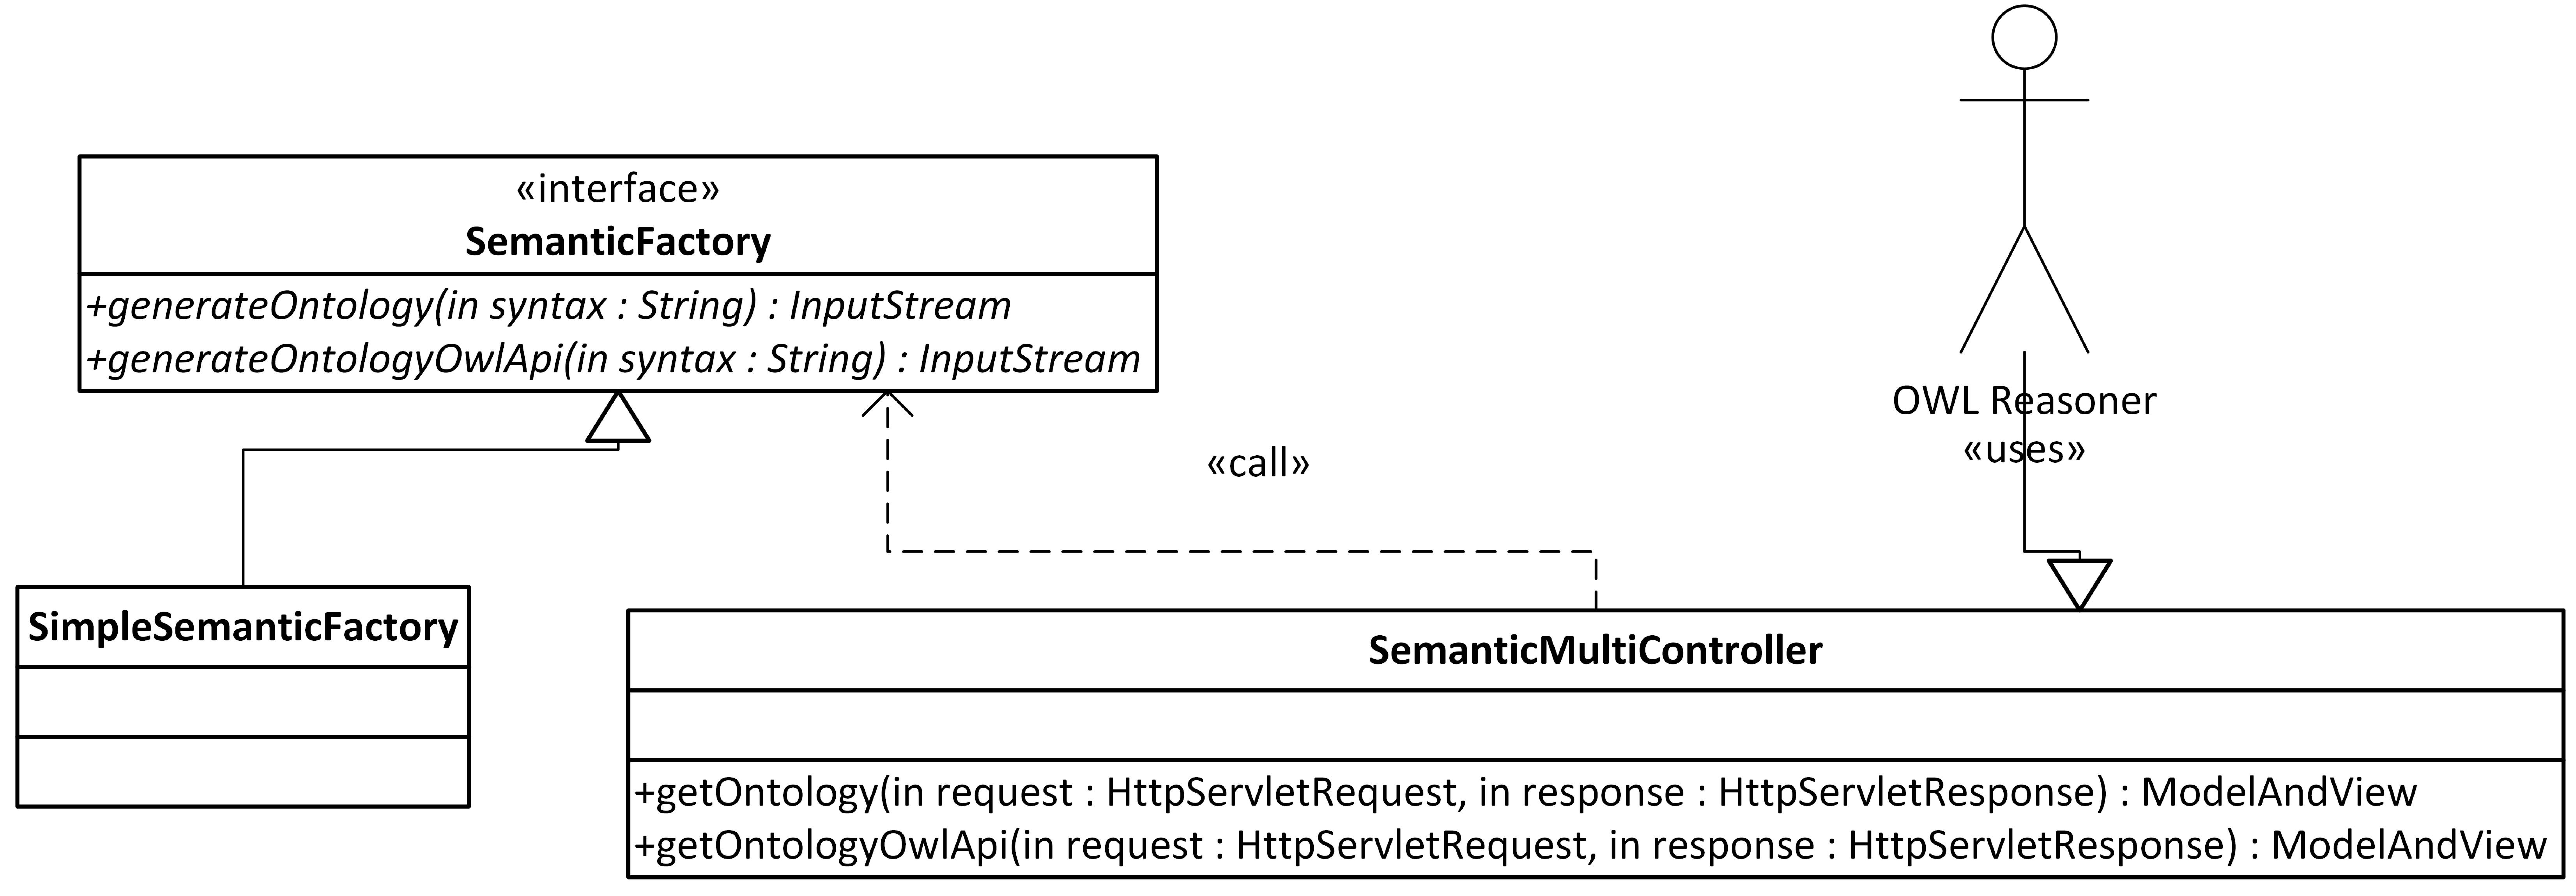
\includegraphics[width=17cm]{SF_integration}
\caption{Semantic Framework Integration. A user (e.g. OWL reasoner) calls the \emph{SemanticMulticontroller}. This controller has two methods, \emph{getOntology} and \emph{getOntologyOwlApi}. A~required output syntax is passed to the methods as a part of the HttpServletRequest parameter. The Semantic Framework is called through the \emph{SemanticFactory} Interface.}
\label{fig:Semantic_Framework_Integration}
\end{figure}

%\subsubsection{Registration within the Neuroscience Information Framework}
%\label{Registration_within_nif}

The generated OWL documents are typically used when registering the EEG/ERP Portal with other providers of neuroinformatics services. We successfully used the Neuroscience Informational Framework (NIF)~\citep{NIF-Neuroinformatics}. The NIF framework provides a unified interface for accessing neurophysiological data through resources described by ontology web languages~\citep{springerlink:10.1007/s12021-008-9033-y}. NIF uses a~proprietary framework \emph{DISCO} \citep{Marenco2010}. It is an XML-based script containing a static description of the registered resource. The dynamic content is accessed through a generated ontology. The structure of metadata instances is stored in an \emph{Interoperability XML} file that is a part of the DISCO protocol. The interoperability file is stored in the root directory of the EEG/ERP Portal together with generated DISCO files. The NIF framework reloads it at regular intervals. It enables dynamic access to the content of the EEG/ERP Portal. Figure \ref{fig:NIF_registry_preview} shows experiments listed through the NIF registry. Currently more then 100 experiments are available in the NIF registry and new ones are gradually being added.

\begin{figure}
\center
  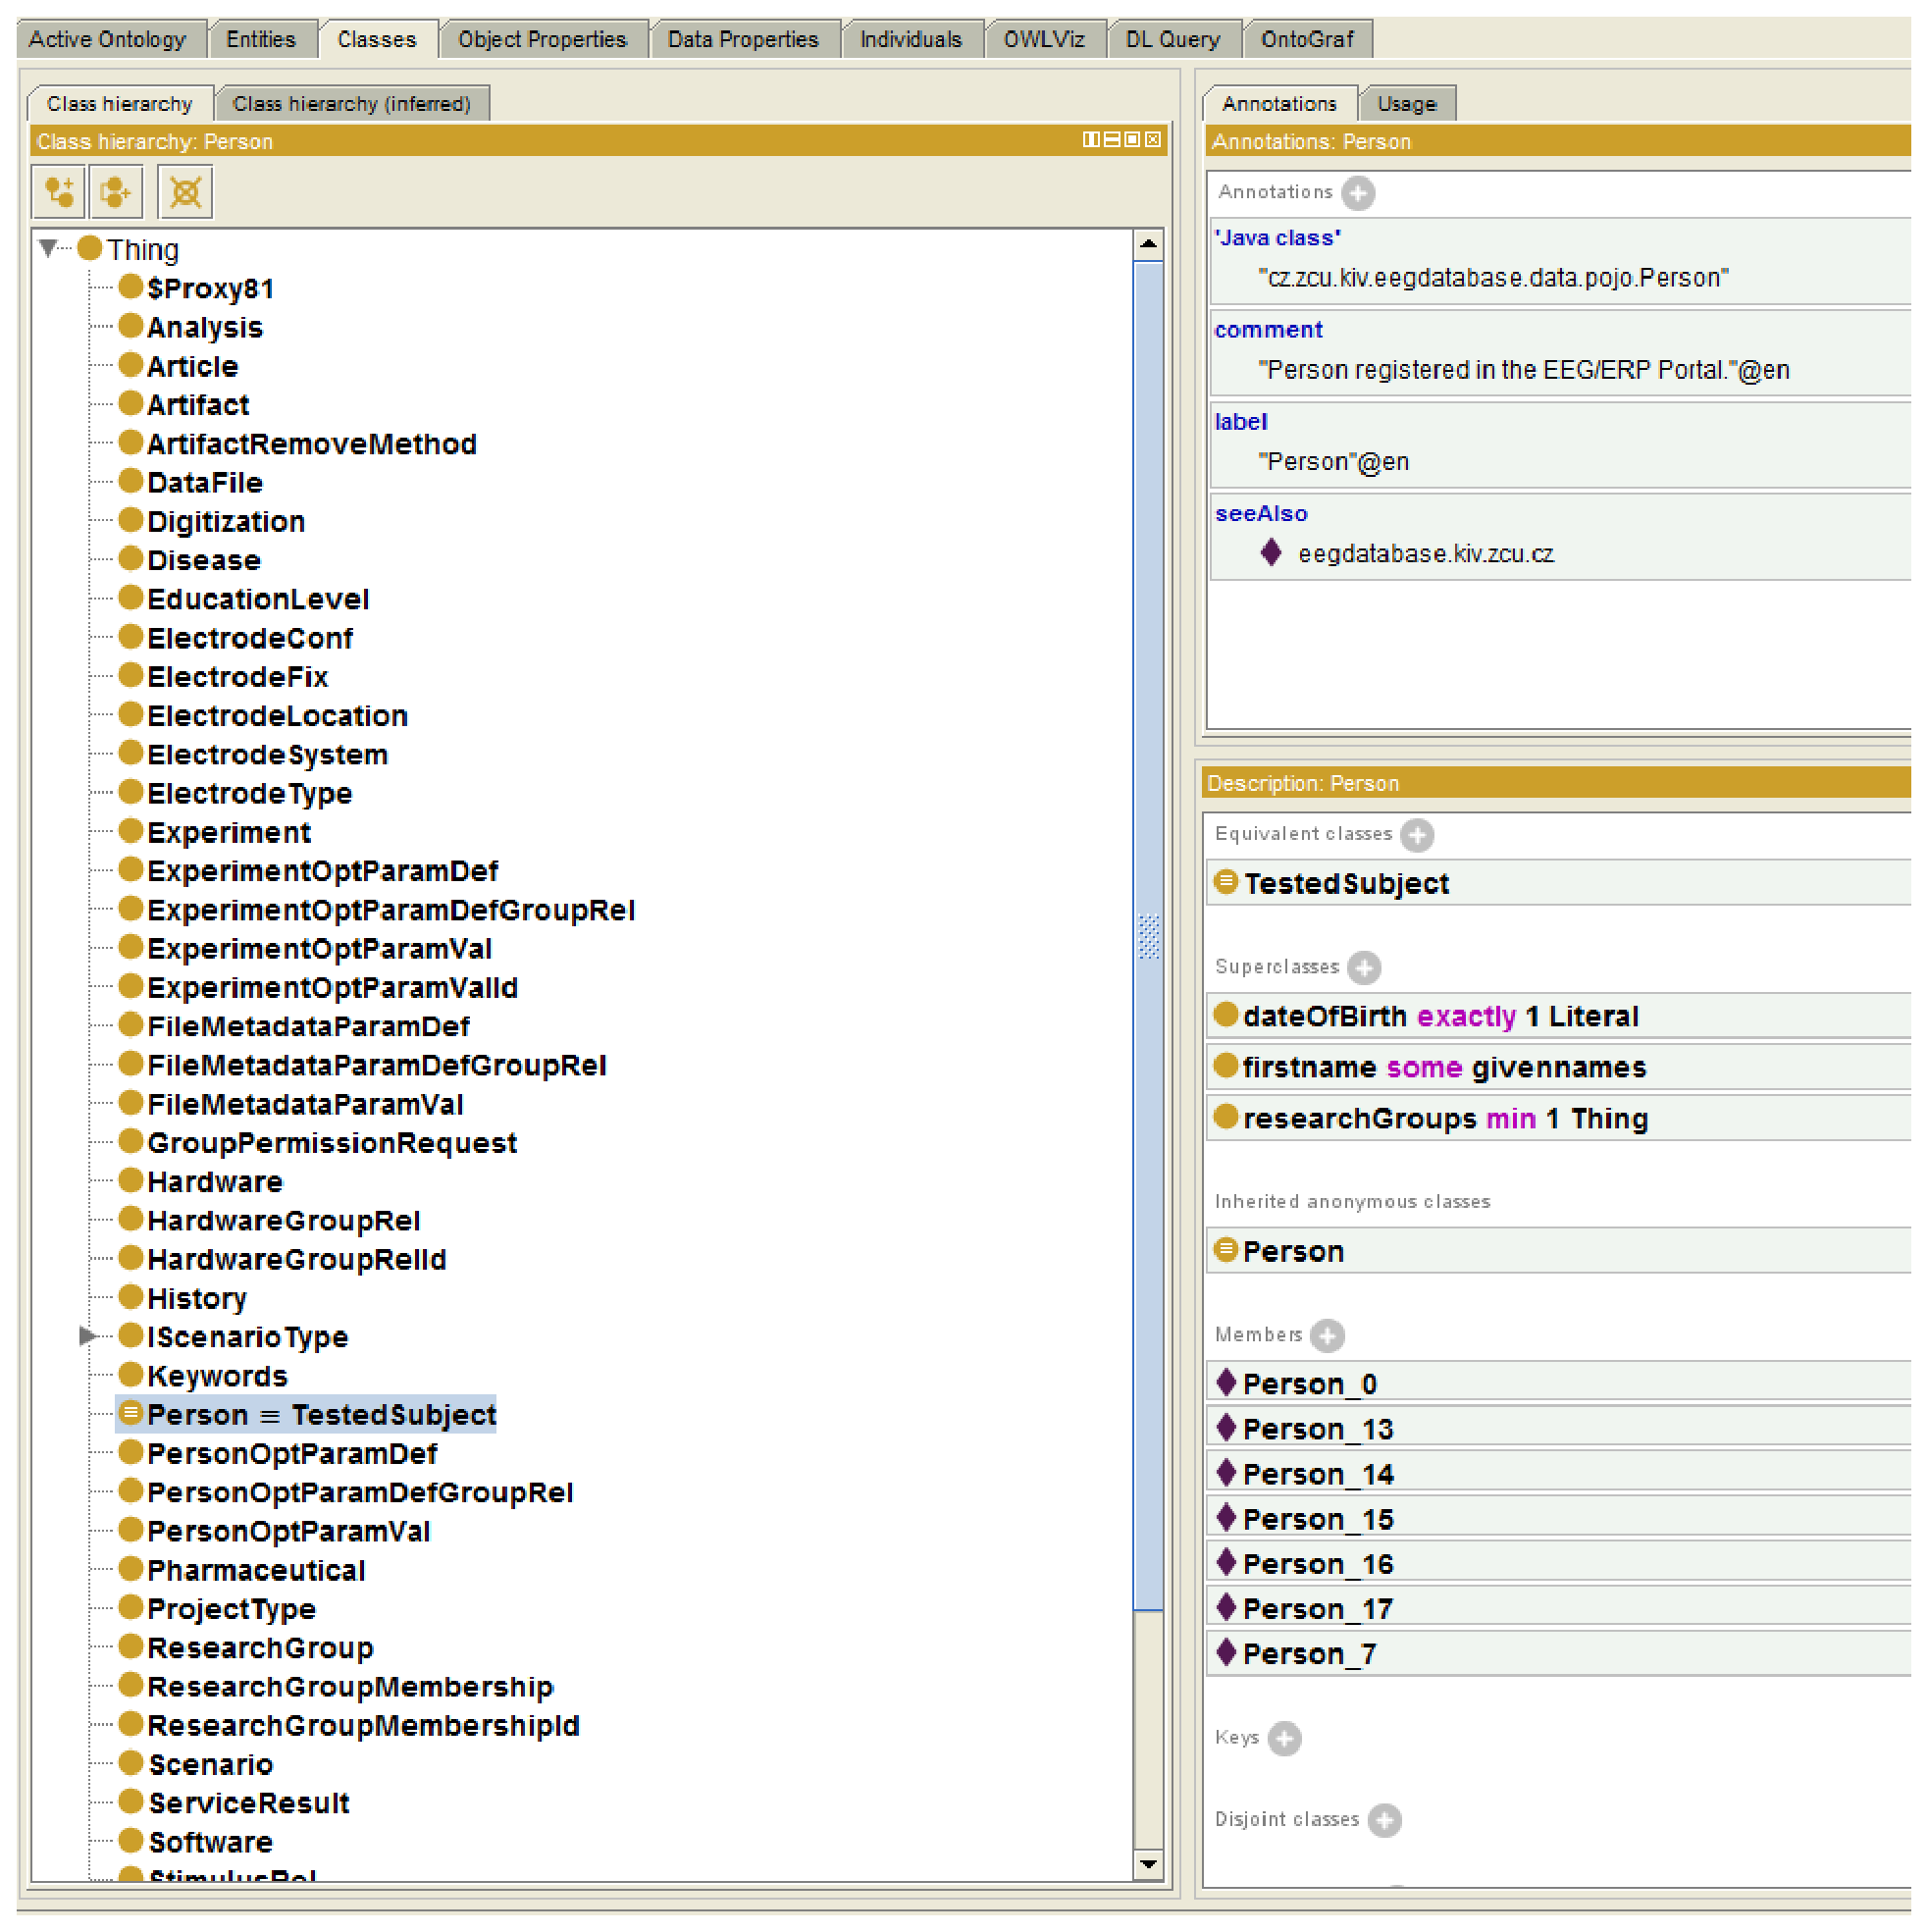
\includegraphics[width=17.5cm]{protege_loaded_ontology}
\caption{Prot\'{e}ge Visualization. The left column shows ontology classes. All classes are subclasses of a superclass \emph{Thing}. The right window shows the marked class \emph{Person}, the class annotations transformed from the enriched JavaBean (e.g. \emph{Comment} or \emph{EquivalentClass}), properties annotations transformed from the enriched JavaBean (e.g. \emph{researchGroup} - each person is a member of at least one research group} and class instances.
\label{fig:visualized_portal_ontology}
\end{figure}

\begin{landscape}
\begin{figure}
  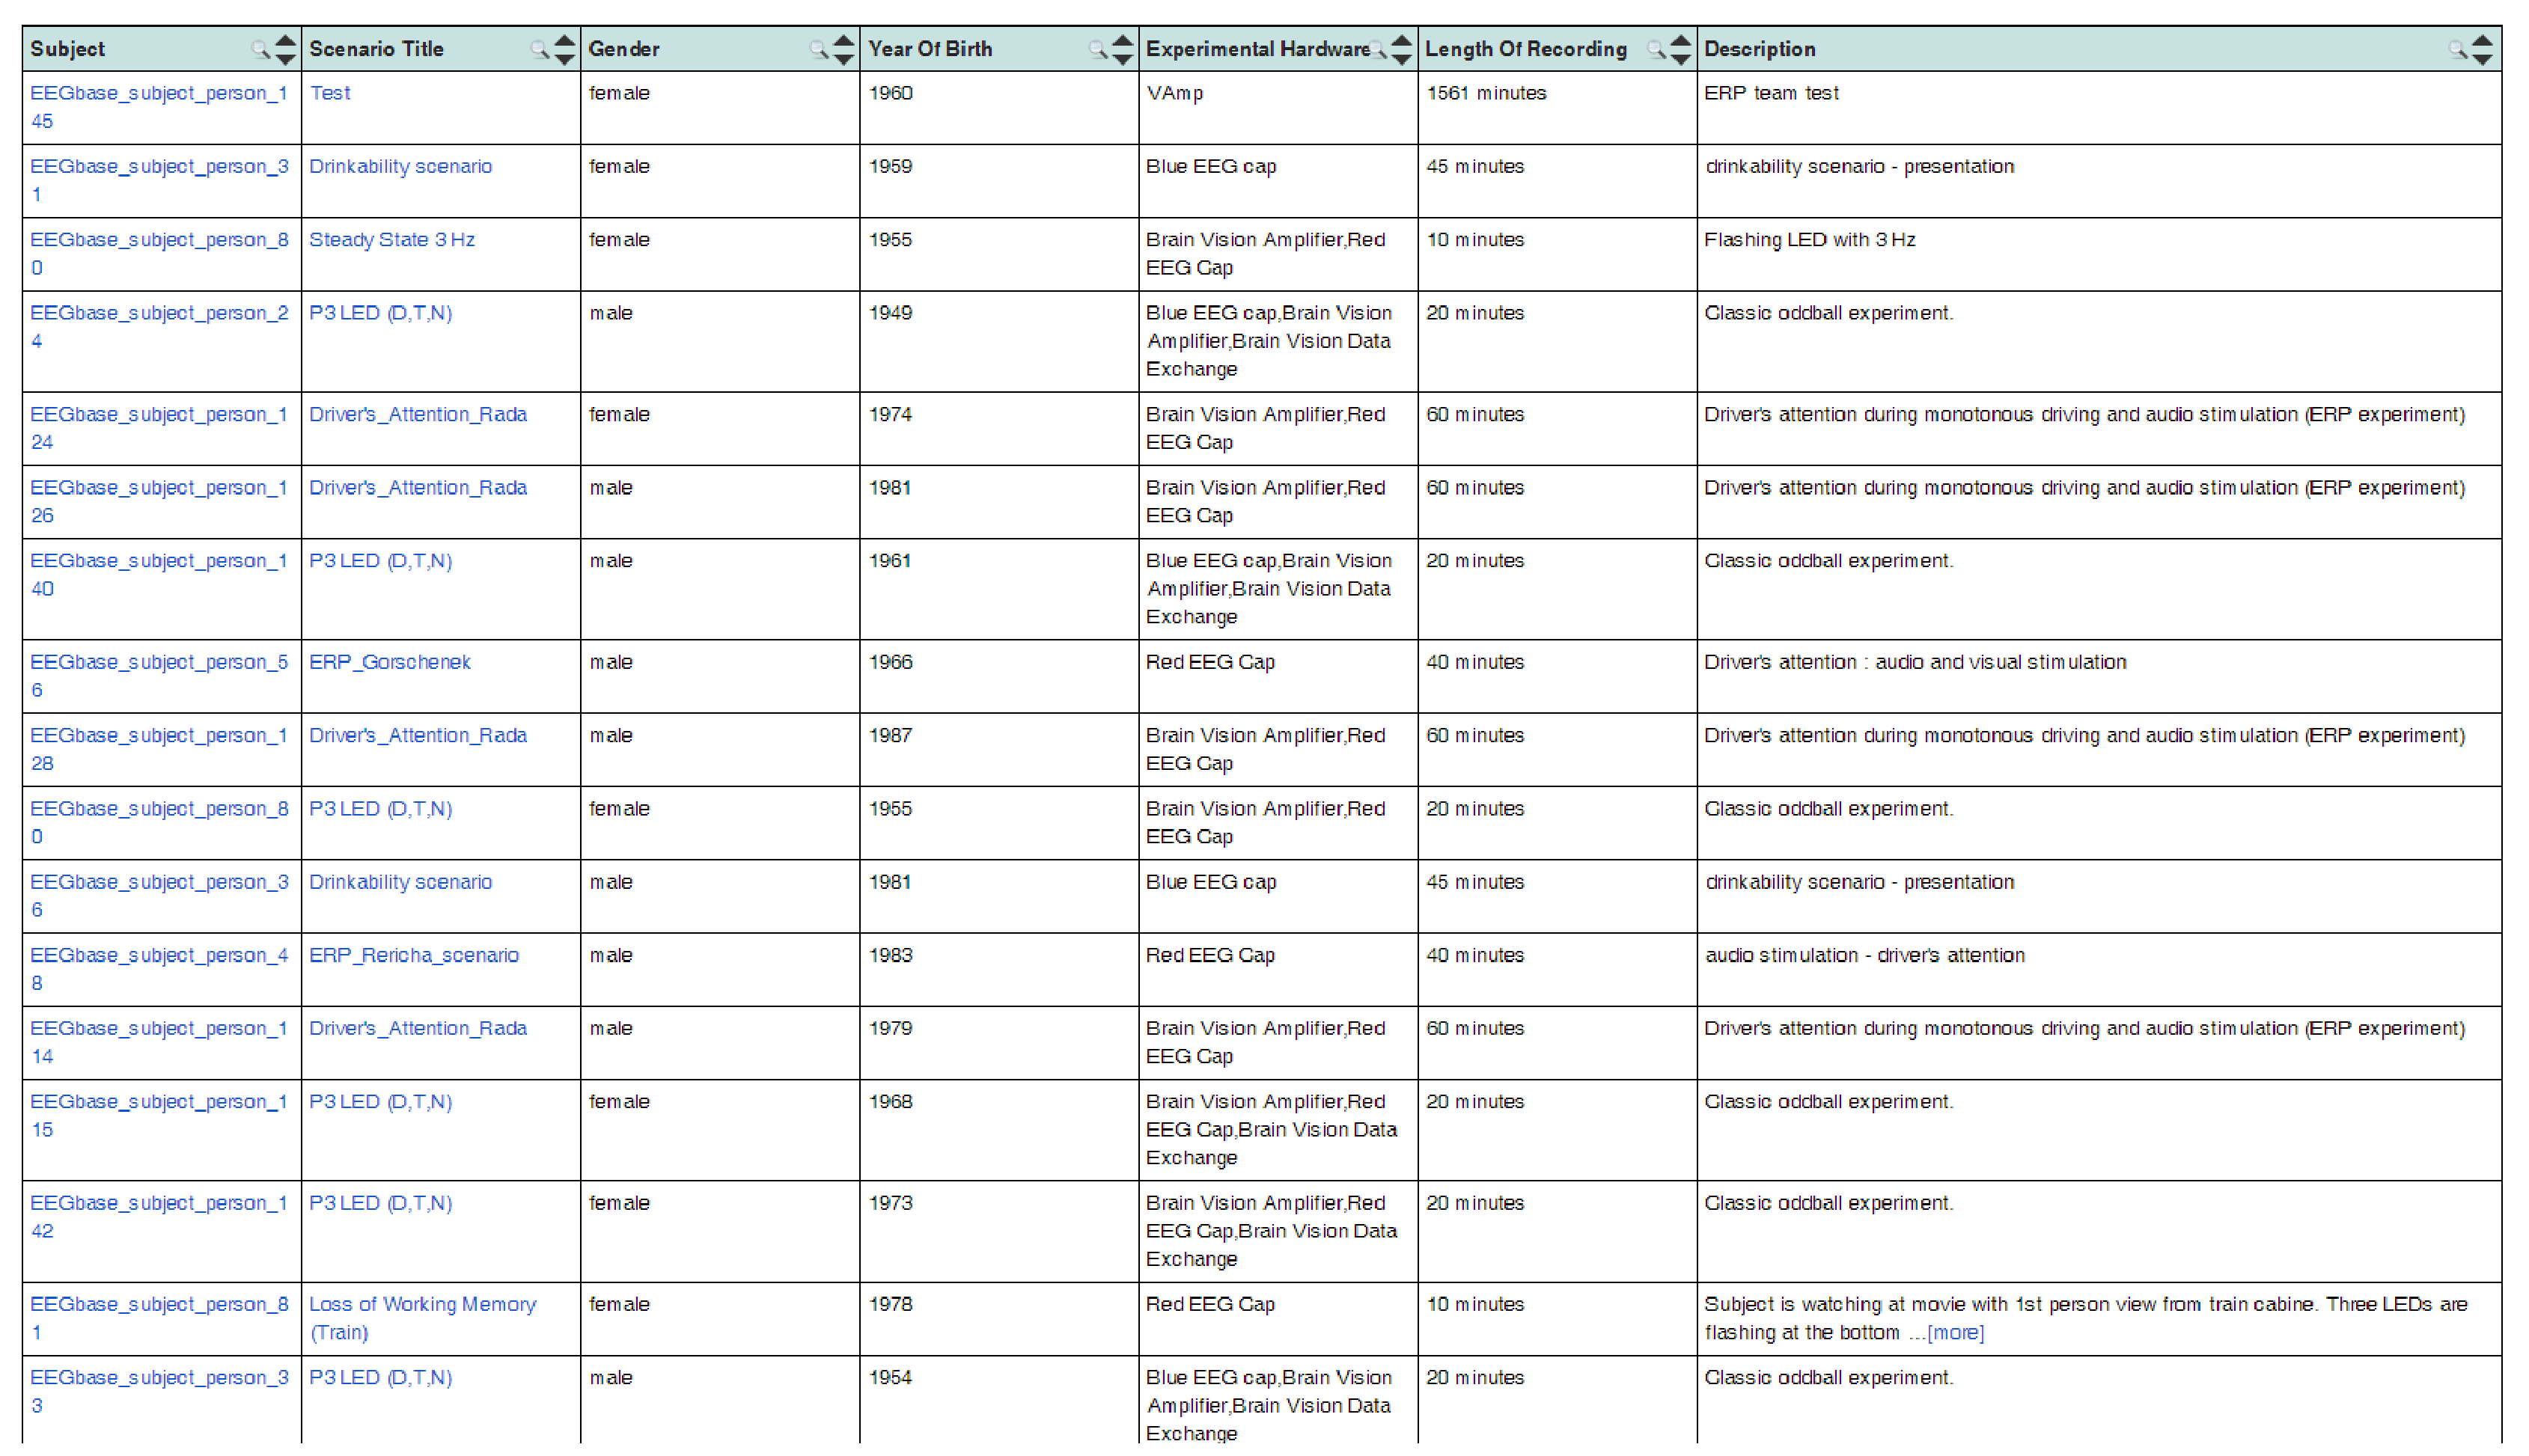
\includegraphics[width=22cm]{nif_preview}
\caption{EEG/ERP Portal in the NIF Registry. The list of experiments stored in the EEG/ERP Portal is shown in the NIF registry at link \protect\url{https://www.neuinfo.org/mynif/search.php?q=eegbase&t=indexable&list=cover&nif=nif-0000-08190-1}. The list contains direct hyperlinks to the experiments stored in the EEG/ERP Portal. When a user clicks on a hyperlink, he/she is redirected to the EEG/ERP Portal.}
\label{fig:NIF_registry_preview}
\end{figure}
\end{landscape}


\section{DISCUSSION}
\label{DISCUSSION}

This article described the possible approaches to the semantic enrichment of structured electrophysiology data. Different views of web engineering and knowledge representation communities on data modelling, necessary scope of semantic descriptions, and used languages and technologies were briefly introduced. The Semantic Web has become (after 13 years of its existence) a certain connection between these communities. Currently, the real benefits of the Semantic Web can be found in the concept of linked data that is already technologically well supported. However, in general the Semantic Web technologies are not mature, often computationally demanding and the community of developers and administrators who would develop/maintain/administrate them is significantly smaller then communities interested in "conventional" programming languages and tools. On the other hand, it is worthwhile to use and promote the Semantic Web languages, standards and technologies that can bring to the real neuroinformatics applications the opportunity to use their higher semantic expressivity.

Based on these assumptions we developed a~software prototype, the Semantic Framework library, that connect conventional technologies and programming tools (relational database, domain-independent Java-based systems) with the languages and technologies of the Semantic Web (RDF, OWL, JenaBean, Jena, OWL API). The most important contribution is a transformational mechanism that maps common JavaBeans accessing data stored in a~relational database into OWL individuals. In addition, the semantic diversity that exists due to the different semantic expressivity of the object-oriented model and the Semantic Web languages was partly addressed using a custom annotation-based approach. Java annotations are enriched by additional semantic constructions that are also transformed to the resulting OWL ontology document. This approach using annotations replaces the traditional modeling of ontologies in an~ontological language. The Semantic Framework was integrated in the EEG/ERP Portal and enabled dynamic generation of the output ontology document. This document is used by the Neuroscience Information Framework to provide a~content of the EEG/ERP Portal through its interface.

Although it is difficult to predict the future development of the Semantic Web, at least it can be expected that new proposals for standards will appear and the software tools that will be developed become more mature and stable. These predictions concerning the future development of the Semantic Web (and standards and tools for semantic descriptions in general) are important for our decisions regarding the development of the EEG/ERP Portal and the Semantic Framework itself.

One of the possible challenges is replacement of the relational database with a~NoSQl database for storing experimental metadata. Relational-databases are inflexible when structure modifications are required, while NoSQL databases provide higher scalability and availability because of their free schema. NoSQL databases having key-value organization can easily store RDF triples~\citep{Papailiou:2012:HAQ:2187980.2188058}. There are initiatives (e.g.~\citep{Combining-Relational-and-Semi-structured-Databases-for-an-Inquiry-Application}) that investigate the transformation of a~common relational database to a~NoSQL database. Currently we replaced a~part of the relational database for the NoSQL database ElasticSearch.

Another challenge is to integrate a~standardized data format and metadata structures into the EEG/ERP Portal. We participate in these standardization activities within INCF Electrophysiology Task Force and within the group developing an~experimental ontology for neurophysiology~\citep{OEN}. Even the partial outcomes of these groups are continuously integrated into the EEG/ERP Portal.

Although the presented approach was used and tested in the electrophysiology domain, the mapping mechanism implemented in the Semantic Framework can be easily applied to other domains.

\section{\uppercase{Acknowledgements}}\label{acknowledgements}

This work was supported by the European Regional Development Fund (ERDF), Project "NTIS - New Technologies for Information Society", European Centre of Excellence, CZ.1.05/1.1.00/02.0090.

%\section{Information Sharing Statement}
%\label{Information_sharing_statement}

%The tools, including the EEG/ERP Portal and the Semantic Framework, are distributed under the GNU Public License. Both are hosted in GitHub repositories. The EEG/ERP Portal is under the INCF group (\url{https://github.com/INCF/eeg-database}) and the Semantic Framework is under the neuroinformatics group of our department (\url{https://github.com/NEUROINFORMATICS-GROUP-FAV-KIV-ZCU/Semantic-Framework}). The EEG/ERP Portal is available on \url{http://eegdatabase.kiv.zcu.cz}.

\bibliographystyle{frontiersinSCNS&ENG} % for Science and Engineering articles
%\bibliographystyle{frontiersinMED} % for Medicine articles
\bibliography{semantic-framework}
\end{document}
